\documentclass[twoside,12pt]{latex/classes/libro}
\usepackage{amsmath}
\begin{document}

\frontmatter
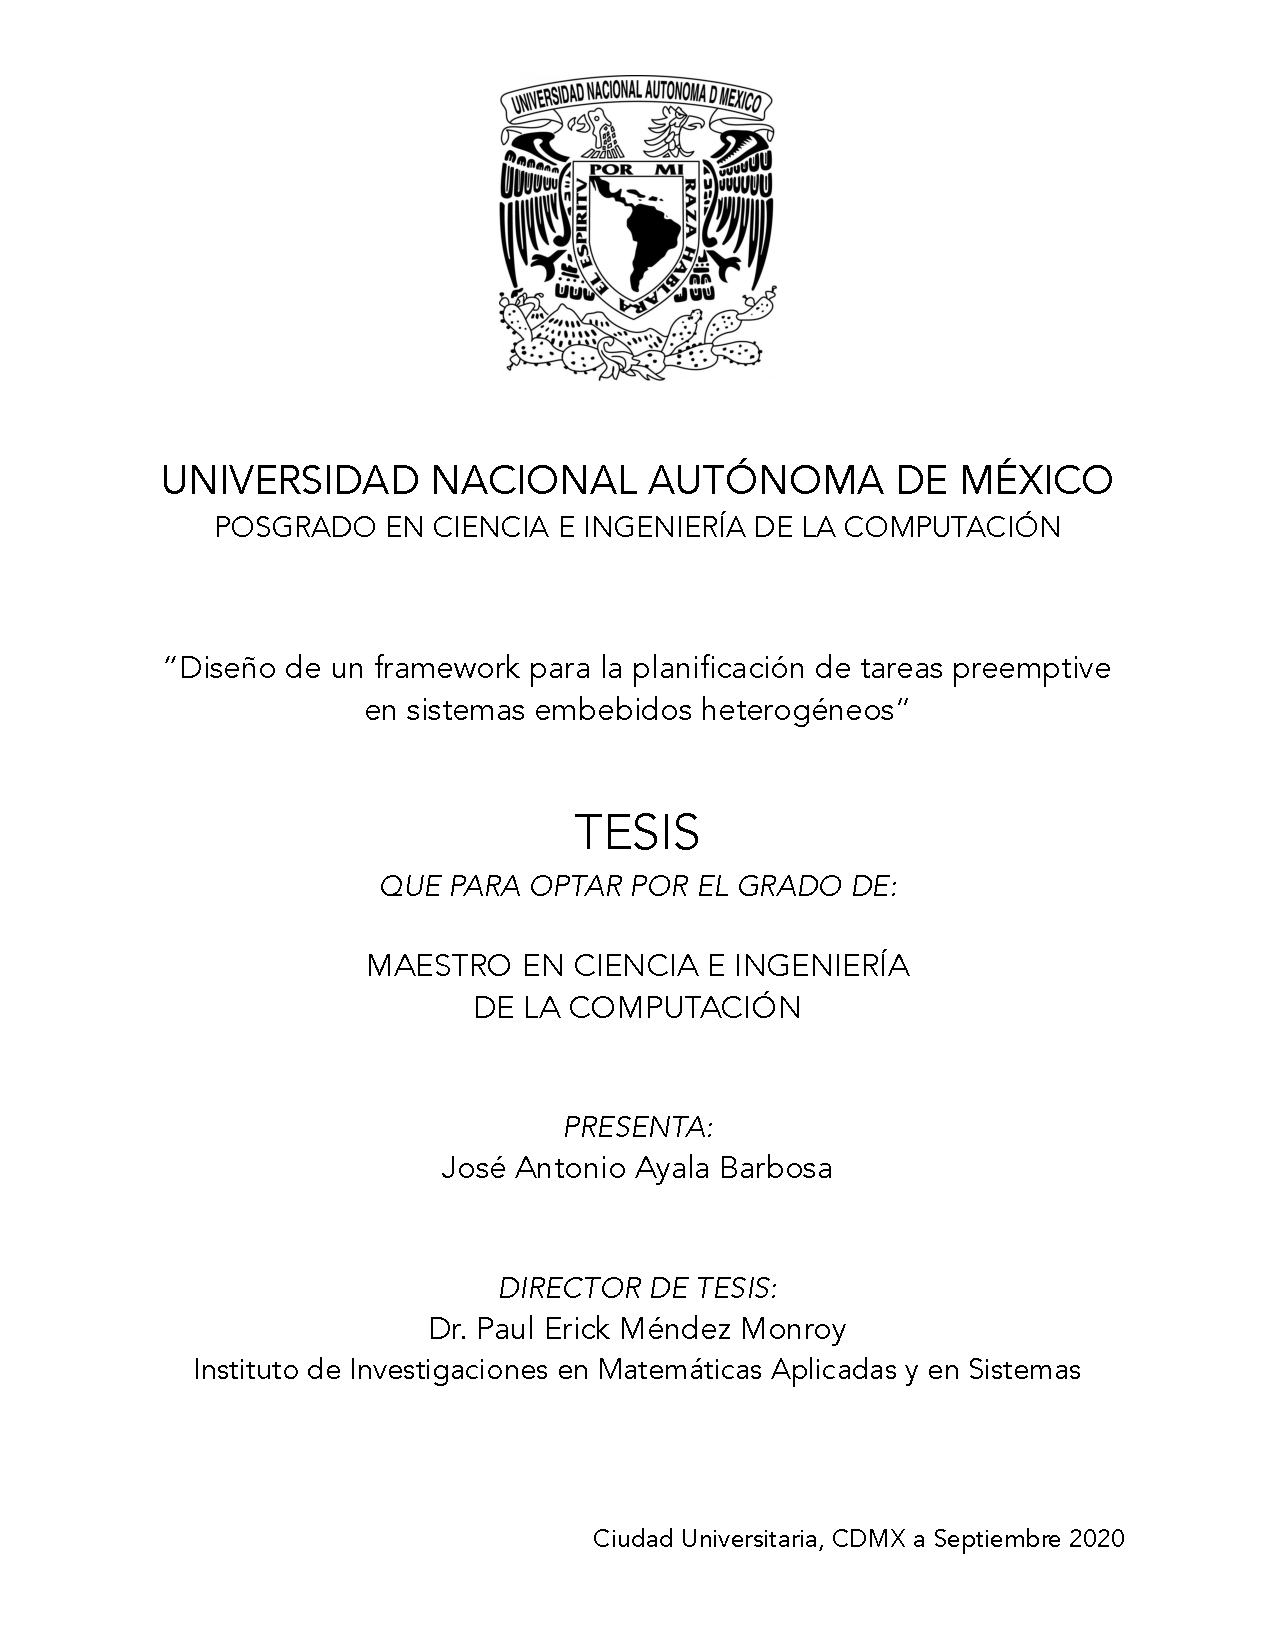
\includepdf{0_frontmatter/portada_Oficial.pdf}
%\graphicspath{{0_frontmatter/figures/}}

\thispagestyle{empty}
\newgeometry{top=4cm,bottom=2.54cm}
\begin{changemargin}{-1cm}{-1.5cm}
  \fcolorbox{white}{white}{
    \begin{minipage}[c][0.16\textheight][c]{0.2\textwidth}
      \begin{center}
        
\includegraphics[scale=0.19]{escudo}
      \end{center}
    \end{minipage}
  }
  \fcolorbox{white}{white}{
    \begin{minipage}[c][0.16\textheight][t]{0.82\textwidth}
      \begin{center}
        \textbf{\Large UNIVERSIDAD NACIONAL AUTÓNOMA DE MÉXICO}
        \vspace{.5cm}
        \hrule height2.5pt
        \vspace{.1cm}
        \hrule height1pt
        \vspace{.9cm}
        \textbf{\Large\scshape División de Estudios de Posgrado}
      \end{center}
    \end{minipage}
  }

  \fcolorbox{white}{white}{
    \begin{minipage}[c][0.75\textheight][t]{0.2\textwidth}
      \begin{center}
        \hskip2pt
        \vrule width2.5pt height16cm
        \hskip1mm
        \vrule width1pt height16cm
      \end{center}
    \end{minipage}
  }
  \fcolorbox{white}{white}{
    \begin{minipage}[c][0.75\textheight][t]{0.82\textwidth}
      \vspace{8mm}
      \begin{center}
        \textbf{\Large \scshape {Posgrado en Ciencias e Ingeniería de
            la Computación}}

        \vspace{1.2cm}

        \makebox[5cm][c]{\Large \textbf{TESIS}}  \\\vspace{5mm}
        {Diseño de una metodología para la migración de aplicaciones web en Java a microservicios}\\
        \vspace{5mm}
        \textit{QUE PARA OBTENER EL T\'ITULO DE:}\\\vspace{5mm}
        {{\scshape{\textbf{\Large{Maestro en Ciencia e Ingeniería
                  en Computación}}}}}\\[30pt]
        PRESENTA:\\[5pt]
        \Large{\textbf{\scshape{Ing. Carlos Eduardo Romero Casanova}}}\\
        \vspace{1cm}
        {{\textit{\normalsize{DIRECTOR:}}}\\[5pt]
          \textbf{\scshape{M. C. Gustavo Arturo Márquez Flores}}}
        \vspace{2cm}
        \begin{flushright}
          \small{{Ciudad de México,}{ }{\today}}
        \end{flushright}
      \end{center}
    \end{minipage}
  }
\end{changemargin}
\restoregeometry{}
\clearpage

~\vfill
\thispagestyle{empty}

\noindent \textsc{Posgrado en Ciencia e Ingeniería de la Computación,\\ Universidad Nacional Autónoma de México}\\

\noindent \textsc{José Antonio Ayala Barbosa}\\

%\noindent Tesis que para optar por el grado de
\noindent Maestría en Ciencia e Ingeniería de la Computación\\
%\noindent \textit{Primera Edición, \today}\\
\noindent \textit{\today}\\
\\
Este trabajo fue apoyado por los proyectos UNAM-PAPIIT IA104218, IA102620
%\begin{prefacio}

.......................

\end{prefacio}
\pagestyle{empty}
\begin{agradecimiento}

  A mis padres
  
  
  A mis amigos
  
  
  A la UNAM
  
  
  A CONACYT
  

\end{agradecimiento}
\tableofcontents
\cleardoublepage
\listoffigures
\listoftables
\lstlistoflistings
\cleardoublepage

\mainmatter
%%Latín
% e.g.    -> por ejemplo (analogias o ejemplos para generar contexto)
% et al. -> y otros (para autores)
% i.e.    -> es decir  (explicación más detallada)


%Introducción
\chapter{Introducción}
\label{cha:Introducción}

\graphicspath{{figures/}}

Las tecnologías emergentes, en especial la de los vehículos autónomos, requieren de soluciones de cómputo intensivo. Cada vez más empresas aceleran sus aplicaciones embebidas mediante la GPGPU con el fin de solventar estas demandas de recursos. Desafortunadamente, las GPUs carecen de soporte para aplicaciones en tiempo real, por ejemplo de soporte preemtive, el cual limita su aplicabilidad en el dominio de sistemas embebidos.

Las GPU modernas se adoptan ampliamente en muchos entornos multitarea, incluidos los centros de datos y los teléfonos inteligentes. Sin embargo, el soporte actual para la programación de múltiples GPU
los núcleos (de diferentes aplicaciones) son limitados, formando una gran barrera para que la GPU satisfaga muchas necesidades prácticas.

La administración predeterminada de GPU es a través de los controladores de GPU no revelados y sigue una política de orden de llegada first-come-first-serve.

Los sistemas en tiempo real deben reaccionar dentro de limites de tiempo precisos para garantizar una corrección funcional, satisfacer los criterios de calidad o evitar daños críticos.

Utilizamos la terminología de CUDA para nuestra discusión, pero tenga en cuenta que el problema y la solución discutidos en este documento también se aplican a otros modelos de programación de GPU (por ejemplo, OpenCL).



\section{Problema y Oportunidad}
En la mayoría de las organizaciones que emplean sistemas en tiempo real hay una creciente necesidad por la adopción de una tecnología más flexible como lo es la incorporación de sistemas con tareas preemptive.

Aunque dicha implementación es poco investigada actualmente en la literatura, este trabajo de tesis nos brinda la oportunidad de idear las bases de un framework que facilite el diseño y/o desarrollos de aplicaciones en tiempo real, y específicamente, con tareas preemptive.

\section{Hipótesis}
La hipótesis del presente trabajo es:

\begin{quote}
\textit{Es posible diseñar un framework que permita la ejecución de tareas en modo preemptive sobre sistemas embebidos heterogéneos para una mejor administración de sus recursos de cómputo.}
\end{quote}

\section{Aproximación}

Mediante el análisis de los elementos inherentes a la estructura de ejecución de procesos híbridos (CPU + GPU) que corren sobre un sistema embebido heterogéneo en particular, se realiza un diseño de la arquitectura del framework que permite la utilización de tareas preemptive.

\section{Contribuciones}
Tener las bases del diseño de un framework que permita planificar la ejecución de tareas preemptive, ya que al implementar puntos preemptive en planificación estática y dinámica se pueden disminuir los plazos vencidos de tareas con alta prioridad y mejorar el desempeño general del sistema.

\section {Estructura de la tesis}

El presente trabajo se estructura en cinco capítulos, en el capítulo \textbf{Antecedentes}, se da una introducción a los conceptos que forman partes del marco teórico, y que son necesarios para entender el contexto en el que se desenvuelve el trabajo. En el capítulo \textbf{Trabajo Relacionado}, se da un breve resumen sobre los textos que contienen información pertinente del estado del arte del tema. Posteriormente, se encuentra el capítulo \textbf{Diseño del framework} en donde se describe puntualmente la propuesta de solución. Finalmente, en el capítulo \textbf{Conclusiones y Trabajo Futuro} se recapitulan los alcances del trabajo y se mencionan los puntos que se dejaron para un trabajo futuro,


    %CPU y GPU -> femeninos
    %Schedule -> planificación
    %Preemptive -> preventivo
    %Preemption -> prevención
    %----------------------------------------------------------------------
\chapter{Antecedentes}
    \label{cha:Antecedentes}

     %INGENIERIA DE SOFTWARE
     \section{Ingeniería de Software}

 El Instituto de Ingeniería Eléctrica y Electrónica (Institute of Electrical and Electronics Engineers – IEEE) define a la Ingeniería de Software como:

\begin{quote}
\textit{"La Ingeniería de Software es la aplicación de un enfoque sistemático, disciplinado y cuantificable al desarrollo, operación y mantenimiento de software; es decir, la aplicación de la ingeniería al software.\cite{IeeeSG}"}
\end{quote}

La Ingeniería de Software aplica diferentes técnicas, normas y métodos que permiten obtener mejores resultados al desarrollar y usar piezas software, al tratar con muchas de las áreas de Ciencias de la Computación es posible llegar a cumplir de manera satisfactoria con los objetivos fundamentales de la Ingeniería de Software. Entre los objetivos de la Ingeniería de Software están\cite{enSWE}:

\begin{itemize}
\item Mejorar el diseño de aplicaciones o software de tal modo que se adapten de mejor manera a las necesidades de las organizaciones o finalidades para las cuales fueron creadas.
\item Promover mayor calidad al desarrollar aplicaciones complejas.
\item Brindar mayor exactitud en los costos de proyectos y tiempo de desarrollo de los mismos.
\item Aumentar la eficiencia de los sistemas al introducir procesos que permitan medir mediante normas específicas la calidad del software desarrollado, buscando siempre la mayor calidad posible de acuerdo a  las necesidades y los resultados que se deseen generar.
\item Una mejor organización de equipos de trabajo, en el área de desarrollo y mantenimiento de software.
\item Detectar a través de pruebas, posibles mejoras para un mejor funcionamiento del software desarrollado.
\end{itemize} 

     \subsection{Framework}
Un framework o marco de trabajo es la estructura y metodología que se establece para normalizar, controlar y organizar, ya sea, una aplicación completa, o bien, una parte de ella. 
Esto representa una ventaja para los participantes en el desarrollo del sistema, ya que automatiza procesos y funciones habituales, además agiliza la codificación de ciertos mecanismo ya implementados al reutilizar código.
Un framework puede ser considerada como un molde configurable, al que podemos añadirle atributos especiales para finalmente construir una solución integrada.
\newline

La utilización de un framework siempre conlleva una curva de aprendizaje, pero a largo plazo facilita la programación, escalabilidad y el mantenimiento de los sistemas.
		
    %SISTEMAS EN TIEMPO REAL
    \section{Sistemas en tiempo real}\label{sec:sistr}

    Los sistemas en tiempo real son sistemas de cómputo cuyas tareas deben actuar dentro de limitaciones de tiempo precisas ante eventos en su entorno. Por lo que el comportamiento del sistema depende, no sólo del resultado del cálculo, sino también del momento (tiempo) en que se produce \cite{Buta2011}.
    \newline 
    
    Un sistema en tiempo real debe  responder a entradas generadas dentro de un periodo de tiempo específico para evitar posibles fallas. El deadline o plazo límite es el momento justo antes en que la tarea debe completar su ejecución. Existen tres tipos de plazos: 
%time constrains: plazos de tiempo
%deadline: plazo límite
\begin{itemize}
\item Soft deadline: En este tipo se pueden superar algunos tiempos límites y el sistema aún puede funcionar correctamente.
\item Firm deadline: Aquí los resultados obtenidos en los plazos vencidos no son útiles, pero los plazos son tolerados frecuentemente.
\item Hard deadline: Si una tarea no se cumple en el plazo límite, se producirán resultados catastróficos. Este tipo de límites se utilizan comúnmente en tareas que realizan operaciones críticas.
\end{itemize}   

\subsection{Tipos de tarea}

Existen tres tipos de tareas que están presentes en los sistemas en tiempo real:

\begin{itemize}
\item Tareas periódicas: Se ejecutan en cada intervalo fijo de tiempo conocido. Normalmente, las tareas periódicas tienen restricciones que indican sus plazos de tiempo.
\item Tareas aperiódicas: Se ejecutan aleatoriamente en cualquier plazo de tiempo y no tienen una secuencia de tiempo predefinida.
\item Tareas esporádicas: Son una combinación de tareas periódicas y aperiódicas, donde, en tiempo de ejecución actúan como aperiódicas, pero la tasa de ejecución es de naturaleza periódica.
\end{itemize}   

La mayoría del tiempo los intervalos de tiempo se dan por el plazo límite de una tarea.

    \subsection{Esquemas de planificación}
    
        \subsubsection{Planificación cooperativa}

En el esquema de planificación \textit{\textbf{cooperativa}} o \textit{\textbf{non-preemptive}} mostrado en la figura \ref{fig:schedcoo}, el planificador asigna las tareas a los nodos de procesamiento disponibles y éstas ocupan los recursos de cómputo durante todo su ciclo de vida.

  \begin{figure}[ht]
      \centering
        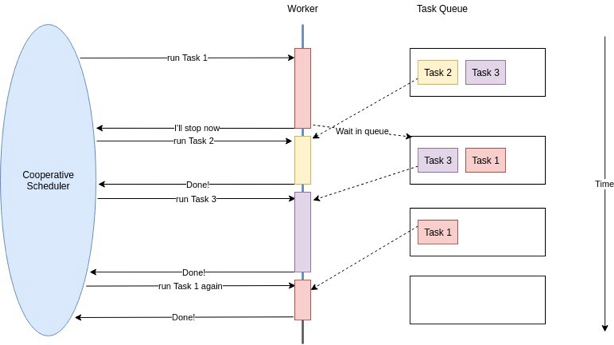
\includegraphics[scale=1]{schedCoo}
        \caption{Planificación cooperativa.\cite{medium}}
        \label{fig:schedcoo}
    \end{figure}
    
Este esquema de planificación es sencillo de implementar ya que las tareas se ejecutarán de manera secuencial, y se implementa cuando se tiene un uso predecible de los tiempos de ejecución de todo el sistema. Pero, como observamos en la figura \ref{fig:schedcoodead}, si una tarea ocupa los recursos en un tiempo superior al contemplado no se puede interrumpir y puede generar plazos vencidos en las demás tareas.

  \begin{figure}[ht]
      \centering
        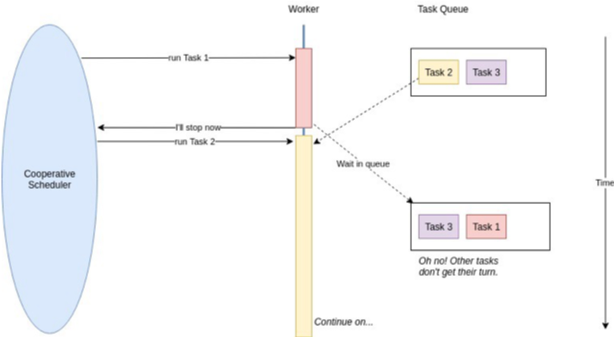
\includegraphics[scale=1]{schedCooDead}
        \caption{Planificación cooperativa con plazos vencidos.\cite{medium}}
        \label{fig:schedcoodead}
    \end{figure}
    
\subsubsection{Planificación preemptive}

En este esquema el planificador asigna las tareas a los recursos disponibles, y les define un tiempo de ejecución máximo, comúnmente llamado quantum\cite{PreeK}. Superado este punto, el planificador interrumpe la tarea para que otra sea ejecutada en su lugar, y la tarea interrumpida debe esperar hasta que le toque su turno nuevamente. Un ejemplo de este esquema, lo tenemos en la figura \ref{fig:schedpree}.

  \begin{figure}[ht]
      \centering
        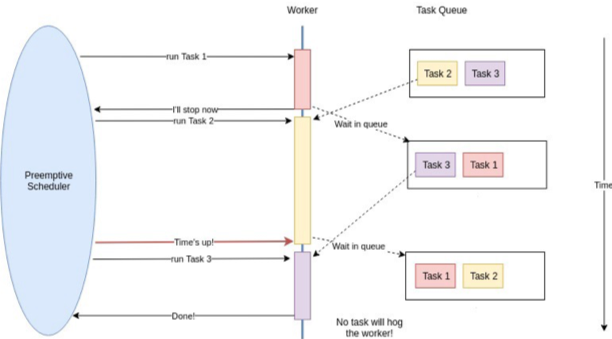
\includegraphics[scale=1]{schedPre}
        \caption{Planificación preemptive.\cite{medium}}
        \label{fig:schedpree}
    \end{figure}

La mayor diferencia entre la planificación cooperativa y la preemptive es que la primera debe ejecutar la tarea de principio a fin, y la segunda puede interrumpir las tareas si así se requiere.
\newline

Debido a que muchas veces se interrumpen tareas a la mitad de un proceso, es necesario almacenar y restaurar el contexto que se tenia antes de dicha interrupción para continuar justo en el punto en donde se quedó. Este proceso de almacenamiento, intercambio y restauración del contexto de las tareas se denomina \textit{cambio de contexto}.
\newline

Como se ha observado, la planificación preemptive actualmente es un requisito para la implementación de los sistemas en tiempo real. Por lo que ha surgido una clasificación dependiendo de su implementación\cite{Buttazzo2013}.

\begin{itemize}
\item \textbf{\textit{Planificación preemptive completa}}. Inmediatamente después de terminar el quantum, se saca de ejecución la tarea actual.
\item \textbf{\textit{Planificación preemptive limitada}}. En la mayoría de los casos, un planificador totalmente preemptive produce suspensiones innecesarias. Para reducir la sobrecarga en tiempo de ejecución, se han propuesto diversas soluciones\cite{Buttazzo2013}:
    \begin{itemize}
    \item \textbf{\textit{Planificación de umbrales preemptive}}.
Esta solución permite que una tarea deshabilite la suspensión preemptive dependiendo del nivel de prioridad. Por lo tanto, a cada tarea se le asigna una prioridad y un threshold preemptive. Por lo que la suspensión preemptive se activa cuando la prioridad de la tarea que llega a la cola de ejecución es mayor que el  threshold de la tarea en ejecución.
    \item \textbf{\textit{Planificación de suspensiones preemptive diferidas}}.
    Cada tarea puede ser ejecutada en un periodo non-preemptive. Aquí cada suspensión se pospone por un periodo determinado de tiempo, en vez de estar específicamente en un lugar en el código. Dependiendo de su implementación puede encontrarse en dos clasificaciones:
        \begin{itemize}
        \item \textbf{\textit{Modelo flotante}}. En este modelo, las regiones non-preemptive son definidas por el programador insertando primitivas específicas en el código que habilitan y deshabilitan el modo preemptive. Dado que el tiempo inicio de ejecución en cada región no se especifica en el modelo, se considera que los puntos están flotando en el código, aunque cumpliendo con una duración que no excede a su quantum.
       
        \item \textbf{\textit{Modelo de activación por triggers}}: Las regiones non-preemptive son activadas por la llegada de una tarea con mayor prioridad y planificadas por un temporizador para durar exactamente su quantum (a menos que terminen antes), después de lo cual se habilita el modo preemptive. Si la tarea en la cola es de menor prioridad, no se interrumpe la que se encuentra en ejecución hasta que termine el siguiente quantum, con lo que se decide si se suspende o continua en ejecución.
        \end{itemize}
    \item \textbf{\textit{Puntos preemptive fijos}}. Una tarea se ejecuta implícitamente en modo non-preemptive y la suspensión sólo se permite dentro de ubicaciones predefinidas dentro del código de la tarea, llamadas puntos preemptive. De esta manera una tarea se divide en varios fragmentos non-preemptive (también llamados subjobs). Si llega una tarea de mayor prioridad entre dos puntos de la que está actualmente en ejecución, la suspensión se pospone hasta el siguiente punto preemptive. 
    \end{itemize}
\end{itemize}


\subsubsection{Clasificación de soporte preemptive}

\label{claspree}
Existen diversas clasificaciones en que se pueden agrupar las soluciones para dar soporte a la planificación de tareas preemptive, una de ellas se basa en el tipo de implementación:

\begin{itemize}
\item \textbf{\textit{Basado en Hardware.}} 
	Aquí se utilizan dispositivos de e/s para el cambio o drenado del contexto para implementar las políticas preemptive. 	

\item \textbf{\textit{Basado en Software.}}
	\begin{itemize}
	\item \textbf{\textit{Partición de Kernel.}}
		Aquí los kernels grandes son partidos en subkernels dividiendo sus grids en fragmentos más pequeños. Es decir, en vez de lanzar todos los Threads por Bloque (TB) de un kernel a la vez, sólo se van lanzando fracciones de éste. Este enfoque es útil para núcleos con muchos TB, donde cada TB tienen un tiempo de ejecución corto. Cuando se tienen diversas especificaciones a resolver por un kernel y estas son necesariamente tareas secuenciales por la dependencia de resultados, se implementan puntos preemptive para dividir el kernel en tareas a completar.  
		%Sin embargo, para aquellos con tiempos de ejecución largos, se pueden generar retrasos significativos y posiblemente tiempos en que haya inversión de prioridad, lo que no es aceptable en sistemas en tiempo real. Aunado a esto, este método no es aplicable a los kernels que requieren una sincronización global entre \gls{TB}, ya que el lanzamiento paulatino de los componentes de un grid podrá causar plazos vencidos en las barreras entre cada fragmento.
	
	\item \textbf{\textit{Partición en Trabajos.}}
		Esta técnica es parecida a la anterior, pero los fragmentos se ven como trabajos, se invocan tantos TB como sea posible tenerlos activos al mismo tiempo. Aquí GPU y CPU comparten una variable que se utiliza para señalizar las solicitudes de cambio de contexto entre los threads activos y los detenidos.

	\item \textbf{\textit{Entorno de Scripts.}}	
		Esta técnica permite manejar automáticamente los kernels dependiendo de ciertos parámetros o puntos de control, liberando al programador de realizarlo manualmente. Esta aproximación funciona especialmente para entornos con kernels pequeños, ya que para aquellos que tienen una ejecución larga es necesario cuidar el nivel de granularidad o podría llegarse a plazos vencidos.
		
	\end{itemize}
	%En esta clasificación también debemos agregar otro apartado:

%\begin{itemize}

%\item \textbf{\textit{Partición en Tareas.}}
%	Es similar a la técnica de partición de Kernel, ya que efectivamente se divide el kernel en fragmentos más pequeños de procesamiento de datos. Cuando se tienen diversas especificaciones a resolver por un kernel y estas son necesariamente tareas secuenciales por la dependencia de resultados, se implementan puntos preemptive para dividir el kernel en tareas a completar.  

%\end{itemize}

\end{itemize}
	
Otra clasificación se obtiene de acuerdo a la forma en que se planifican las tareas:

\begin{itemize}

\item \textbf{\textit{Colas masivas en paralelo.}}
	Este apartado está centrado en, ya sea una o varias colas concurrentes que recopilan y distribuyen el trabajo siguiendo la regla \textit{FIFO}, el primero en entrar, el primero en salir. 
	
\item \textbf{\textit{Administración dinámica de memoria.}}
	Se tiene un administrador de memoria que verifica si es posible asignar memoria para una nueva tarea, o cual de las que actualmente se encuentra en ejecución ha superado su espacio definido. 
	
\item \textbf{\textit{Administración dinámica de los núcleos de procesamiento.}}
	Aquí se limita el número de núcleos de procesamiento en tiempo de ejecución de una GPU para una tarea, y el número depende casi siempre de la prioridad de la tarea.

	
\item \textbf{\textit{Planificación por prioridad.}}
	Se utilizan algoritmos de planificación para manejar dinámicamente el cambio de prioridades y maximizar el rendimiento del sistema. La mayoría de las veces este tipo es el más cercano a una implementación completa de tiempo real.
	
\end{itemize}
%Aunque no esta originalmente contemplado, es necesario discriminar entre la administración de la memoria y la administración de los núcleos que una GPU nos va a prestar para realizar el procesamiento. 
%\newline
     
Finalmente, podemos encontrar una clasificación enfocada en la forma en que se implementa la planificación en el código.

\begin{itemize}

\item \textbf{\textit{Modificación de código fuente.}}
	Es necesario que el programador modifique el código del kernel para implementar cada una de las acciones que va a seguir la tarea, desde su inicio, pasando por su interrupción, y hasta su finalización.
	
\item \textbf{\textit{Modificación del API.}}
	En este apartado, se hace una modificación a nivel de las bibliotecas o el compilador, la ventaja es que la aplicación no es modificada manualmente; sin embargo, su utilización muchas veces no está permitida por los administradores.
	
\end{itemize}

    \subsection{Algoritmos de planificación}\label{sec:AlgoPlan}. 
    
    Un algoritmo de planificación es una estrategia en la cual un sistema decide ejecutar una tarea en un momento dado, debe garantizar que se asigne el tiempo suficiente a todas las tareas del sistema para que puedan cumplir su plazo límite en la medida de lo posible.
    
    La planificación en tiempo real se puede dividir en:
    \begin{itemize}
    \item Estática o Fixed Task Priority (FTP):  Todas las prioridades se asignan al diseñar el sistema y éstas se mantienen constantes durante el tiempo de vida de una tarea.
    \item Dinámica o Dyamic Task Priority (DTP): Se asignan prioridades en el tiempo de ejecución, en función de los parámetros de las tareas. Su objetivo es adaptarse al progreso del sistema para buscar la configuración óptima de planificación.
    \end{itemize}   
    
    
        \begin{table}[h!]
      \begin{center}
            \scriptsize
        \begin{tabular}{|m{1.5cm}|m{2cm}|m{2cm}|m{2cm}|m{2cm}|m{3cm}|}
         \hline
        \cellcolor{lightgray}\textbf{Algoritmo} & \cellcolor{lightgray} \textbf{Asignación de prioridad} & \cellcolor{lightgray} \textbf{Criterio de planificación} & \cellcolor{lightgray} \textbf{Preemptive/ Non-preemptive} & \cellcolor{lightgray} \textbf{Utilización de CPU} & \cellcolor{lightgray} \textbf{Eficiencia}  \\ 
         \hline
          \textbf{SJF} & Estática & Tiempo de Ejecución & Non-preemptive & 100\% & Eficiente con tareas de finalización oportuna \\
         \hline
         \textbf{EDF} & Dinámica & Plazo Límite & Preemptive & 100\% & Eficiente en condiciones subcargadas \\
         \hline 
         \textbf{RM} & Estática & Periodo & Preemptive & < 100\% & Eficiente en condiciones sobrecargadas \\
         \hline
          \textbf{DM} & Estática & Plazo Límite Relativo & Preemptive & > a RM & Eficiente \\
         \hline
          \textbf{LLF} & Dinámica & Laxitud & Preemptive & 100\% & Eficiente \\
         \hline
          \textbf{GEDF} & Dinámica & Plazo Límite y Tiempo de ejecución & Non-preemptive & 100\%& Eficiente en ambientes Non-preemptive \\
         \hline
                \end{tabular}
        \caption{Matriz de comparación de algoritmos de planificación.}
        \label{tab:algoTR}
      \end{center}
    \end{table}
    
    \subsubsection{Shortest Job First}
    Shortest Job First (SJF) es el algoritmo de planificación que asigna la prioridad mayor a la tarea con el menor tiempo de ejecución. SJF es el algoritmo más utilizado cuando se comienzan a estudiar los sistemas en tiempo real debido a su simplicidad, ya que minimiza la cantidad promedio de tiempo que cada tarea debe esperar hasta que se complete su ejecución \cite{Tanenbaum}. Este algoritmo funciona únicamente con tareas non-preemptive, por lo que fácilmente puede llegarse a un estado de inanición de tareas que requieren mucho tiempo para completarse si se agregan continuamente tareas pequeñas.
    
    \subsubsection{Earliest Deadline First} 
    Earliest Deadline First (EDF) es un algoritmo con prioridad dinámica, en el que la tarea con el plazo fijo más próximo tiene la mayor prioridad. Este algoritmo es óptimo para implementación sobre un único procesador, y cuando el sistema se encuentra en bajos y moderados niveles de contención de recursos y datos\cite{Liu}.
    %Ya que cuando se sobrecarga el sistema, la mayoría de las tareas obtienen una alta prioridad, lo que termina en un rendimiento disminuido.
\newline
     
    Es un algoritmo muy extendido en sistemas en tiempo real debido a su optimalidad teórica en el campo no-preemptive, aunque al momento de implementarlo en un planificador preemptive el resultado puede acarrear un exceso de ejecución si se toma el peor caso \cite{EmbSysDes}. Es el algoritmo más extendido al momento de realizar los primeros bosquejos de un sistema en tiempo real.
    %Por ello es necesario buscar alternativas de algoritmos que tengan un mejor desempeño en tareas específicas.
    
     \subsubsection{Rate Monotonic}
    Rate Monotonic (RM) es un algoritmo de planificación preemptive con prioridad estática para un solo procesador\cite{Liu}. RM asigna la prioridad más alta a la tarea con el periodo más corto, suponiendo que los periodos sean igual a los plazos \( (P_{i} = D_{i}) \). En caso de que la tasa de demanda sea mayor el periodo sería más corto y, por ende, la prioridad aumentaría. Por ello es óptimo para usarse en tareas periódicas. La mayor limitación de su implementación, es que al utilizar tareas de prioridad fija no siempre se utiliza el 100\%  del CPU, lo que conlleva al posible desperdicio de recursos\cite{RM}.

\subsubsection{Deadline Monotonic}
Deadline Monotonic (DM) es el algoritmo óptimo de planificación con prioridad fija donde las prioridades son asignadas inversamente proporcionales a los plazos fijos, es decir, cuando se cumple que el plazo es menor al tiempo de la tarea \( (P_{i} < T_{i}) \) y el periodo es igual al plazo limite \( (P_{i} = D_{i}) \) podemos ver a RM como un caso especial de DM \cite{NPr}. DM ejecuta en cada instante de tiempo la tarea con el plazo más corto, por lo que si dos o más tareas tienen el mismo plazo límite, la siguiente en ejecutarse debe elegirse aleatoriamente.

\subsubsection{Least Laxity First}
Least Laxity First (LLF) es un algoritmo óptimo de planificación con prioridad dinámica. La laxitud de una tarea está definida como el plazo límite menos el tiempo de ejecución restante, esta laxitud es la cantidad máxima de tiempo que un trabajo puede esperar cumpliendo su plazo límite. En este algoritmo, se otorga la máxima prioridad al trabajo con la menor laxitud, se permite que la tarea actualmente en ejecución sea intercambiada por otra con menor laxitud en cualquier momento \cite{NPr}.
\newline
  
  El punto débil de este algoritmo se presenta cuando dos tareas presentan la misma laxitud, ya que un proceso se ejecutará durante un período corto de tiempo y luego será reemplazado por el otro y viceversa. Con ello, se obtienen numerosos cambios de contexto durante la vida útil de las tareas y el rendimiento del sistema en general se ve reducido. Este algoritmo es óptimo para sistemas con tareas periódicas \cite{ComRTT}.
  
\subsubsection{Gang Earliest Deadline First}
Gang Earliest Deadline First (GEDF) está pensado para mejorar el desempeño de EDF durante condiciones de sobrecarga\cite{GEDF}. La idea principal de su funcionamiento es agrupar las tareas con plazo límite similares y dentro de cada grupo planificar las tareas con SJF \cite{ComRTT}. 
El parámetro rango de grupo (Gr) es un porcentaje de la tarea al comienzo del plazo absoluto de cada cola que determina el ingreso de la tarea a un grupo. Este algoritmo tiene soporte multiprocesador, por lo que en este ambiente resulta más efectivo\cite{GEDF}.

%Aunque existen protocolos más simples y fáciles de implementar, como lo es la planificación non-preemtive, pueden llegar a provocarse bloqueos en el sistema en tareas críticas de seguridad. 

    %----------------------------------------------------------------------
    %GPU
        \section{CPU}
    La unidad de procesamiento central o CPU es un procesador de propósito general, lo cual significa que puede hacer una variedad de cálculos pero está diseñado para realizar el procesamiento de información en serie y consta de pocos núcleos de propósito general. Aunque se pueden utilizar bibliotecas para realizar concurrencia y paralelismo, el hardware \textit{per se} no tiene esa implementación.

     \subsection{Arquitectura del CPU}

Un CPU está compuesto principalmente por:
\begin{itemize}
\item Reloj: elemento que sincroniza las acciones del CPU.
\item ALU (Unidad lógica y aritmética): como su nombre lo indica, soporta pruebas lógicas y cálculos aritméticos, y puede procesar varias instrucciones a la vez.
\item Unidad de Control: se encarga de sincronizar los diversos componentes del procesador.
\item Registros: memorias de tamaño pequeño, del orden de bytes, y que son lo suficientemente rápidas para que el ALU manipule su contenido en cada ciclo de reloj.
\item Unidad de entrada-salida (I/O): soporta la comunicación con las memoria de la computadora y permite el acceso a los periféricos.
\end{itemize}   

\subsection{Núcleos de procesamiento CPU y GPU}
    Es necesario destacar que los núcleos o cores de un CPU y un GPU en principio son similares, pero entre ellos existen diferencias. Un núcleo de CPU es relativamente más potente, está diseñado para realizar un control lógico muy complejo para buscar y optimizar la ejecución secuencial de programas.
\newline
    
    En cambio un núcleo de GPU es más ligero y está optimizado para realizar tareas de paralelismo de datos como un control lógico simple enfocándose en la tasa de transferencia de los programas paralelos.
 \newline
 
        \begin{figure}[ht]
      \centering
        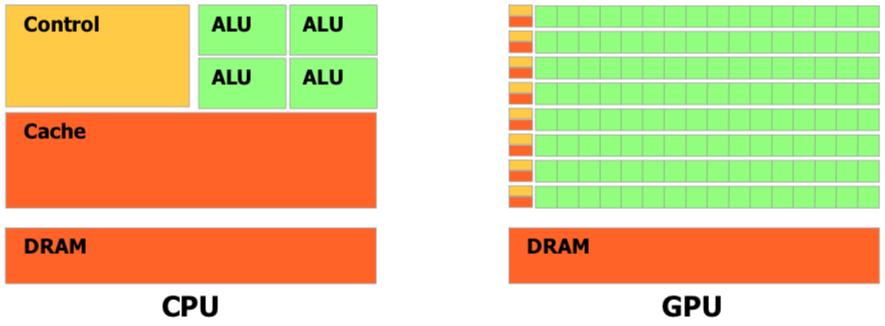
\includegraphics[scale=0.35]{repCPUGPU}
        \caption{Representación de un CPU y un GPU\cite{NCUDA}.}
        \label{fig:repgpgpu}
    \end{figure}

    Con aplicaciones computacionales intensivas, las secciones del programa a menudo muestran una gran cantidad de paralelismo de datos. Las GPU se usan para acelerar la ejecución de esta porción del código. Cuando un componente de hardware que está físicamente separado del CPU se utiliza para acelerar secciones computacionalmente intensivas de una aplicación, se le denomina acelerador de hardware. Se puede decir que las GPU son el ejemplo más común de un acelerador de hardware.

    \section{GPU}
   
    La unidad de procesamiento gráfico o GPU es un procesador especializado para tareas que requieren de un alto grado de paralelismo. Su uso más extendido es el procesamiento de instrucciones aplicadas a campo de imágenes 2D y 3D, realizando cálculos con pixeles y texeles\cite{TX2CU}.
\newline
   
   La tarjeta gráfica en su interior puede contener una cantidad de núcleos de un orden de cientos hasta miles de unidades que son más pequeñas y que por ende, individualmente realizan un menor número de operaciones. Esto hace que la GPU esté optimizada para procesar cantidades enormes de datos pero con programas más específicos\cite{gpgpu}. Lo más común al utilizar la aceleración por GPU es ejecutar una misma instrucción a múltiples datos para aprovechar su arquitectura.
   
    \subsection{Arquitectura GPU}

La arquitectura de las tarjetas gráficas ha experimentado ciertas evoluciones en su desarrollo para permitir a los programadores hacer un uso más eficiente de su poder de procesamiento. Una tarjeta gráfica es básicamente un multiprocesador compuesto de una gran cantidad de núcleos de procesamiento que trabajan en paralelo, junto con los componentes de un CPU. Las GPU incorporan:

\begin{itemize}
\item Memoria: cuentan con diferentes tipos de memoria y principalmente compuesta por el tipo DRAM (Memoria dinámica de acceso aleatorio).
	\begin{itemize}
	\item Memoria global: almacena los datos enviados desde el CPU.
	\item Memoria constante de sólo lectura.
	\item Memoria de texturas de sólo lectura.
	\item Registros locales por núcleo de 32 bits. 
	\end{itemize}
Donde las memorias constantes y de textura son de acceso más rápidas que la memoria global, ya que actúan como una especie de caché.

\item Programación en streams: La arquitectura de una GPU está diseñada con base en la programación de streams, el cual involucra múltiples cálculos en paralelo para un stream de datos\cite{stream}. 

	\begin{itemize}
	\item Stream: Conjunto de elementos que tendrán un tratamiento similar.
	\item Kernel: Tratamiento aplicado a cada elemento del stream.
	\item Thread: Tratamiento ejecutado por procesador aplicado a un elemento del stream.
	\end{itemize} 
%	\item Gather y Scatter: Cuando se aplica un kernel a un stream, este aplica todas sus instrucciones a cada elemento, por lo que cada elemento se almacena en un una posición bien definida dentro de la memoria utilizando índices que auxilian a localizarlo, a esta acción se le conoce como Scatter. 

  %      \begin{figure}[ht]
   %   \centering
    %    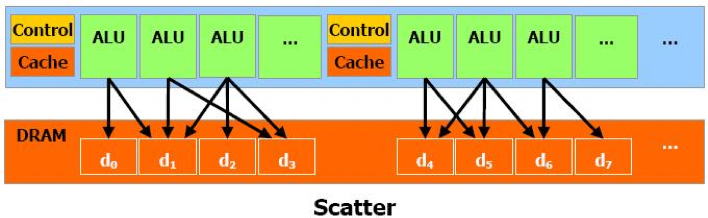
\includegraphics[scale=1]{scatter}
     %   \caption{Escritura en DRAM\cite{NCUDA}.}
      %  \label{fig:scatter}
%    \end{figure}
   
%En cambio, el Gather es la lectura o recolección de un stream en memoria para ser procesado por una unidad de procesamiento.

%        \begin{figure}[ht]
 %     \centering
  %      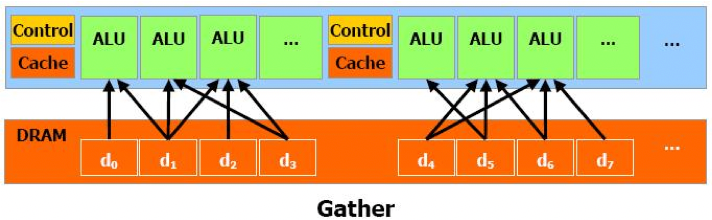
\includegraphics[scale=1]{gather}
   %     \caption{Lectura en DRAM\cite{NCUDA}.}
    %    \label{fig:gather}
    %\end{figure}

\end{itemize} 
    
    \subsection{Arquitectura CUDA}
    CUDA es el acrónimo en inglés de \underline{C}ompute \underline{U}nified \underline{D}evice \underline{A}rchitecture, el cual es una arquitectura de hardware y de software que permite ejecutar programas en las tarjetas gráficas de la marca NVIDIA\cite{CUDAP}.
    \newline
   
    CUDA C es una extensión del estándar ANSI C con varios complementos del lenguaje para utilizar la programación heterogénea, añadiendo APIs sencillas para administrar los dispositivos e/s, memoria y otras tareas. También es un modelo de programación escalable que permite a los programas trabajar transparentemente con un número variable de núcleos de procesamiento.
    \newline
    
    Un programa en CUDA consiste en la mezcla de dos códigos: el host code, que tiene que ver con lo realizado por el CPU, y el device code, que ejecutará la GPU. El compilador de NVIDIA (nvcc) separa ambos códigos durante el proceso de compilación y durante la etapa de enlace las bibliotecas de CUDA se agregan a las funciones que irán al device para poder manipular completamente la tarjeta gráfica.
    \newline
    
    A la hora de hablar de su arquitectura se pueden identificar dos perspectivas dependiendo del nivel de abstracción que se requiera, la del programador o la del hardware.
        
  \subsubsection{Perspectiva del programador}
   
    La tabla \ref{tab:CUDAcomp} muestra sus componentes principales de CUDA desde la perspectiva del programador, y la figura \ref{fig:grid} muestra esquemáticamente el como se conforma el grid de un kernel.
    
     \begin{table}[h!]
      \begin{center}
            \footnotesize
        \begin{tabular}{|m{1.5cm}|m{8.5cm}|}
         \hline
         \cellcolor{lightgray}\textbf{kernel} & Funciones paralelas escritas en el programa que indican que operaciones se realizaran en la GPU.\\ 
         \hline
          \cellcolor{lightgray}\textbf{thread} & Unidad mínima que ejecuta una instancia de un kernel. Tiene su propio id dentro un block, su propio contador de programa, registros, memoria privada, entradas y salidas.\\ 
         \hline  
         \cellcolor{lightgray}\textbf{block} & La agrupación de threads que utilizan memoria compartida.\\ 
         \hline
         \cellcolor{lightgray}\textbf{grid} & Arreglo de blocks que ejecutan el mismo kernel, leen y escriben datos en memoria global.\\ 
         \hline
           \end{tabular}
        \caption{Componentes de CUDA para el programador.}
        \label{tab:CUDAcomp}
      \end{center}
    \end{table}
    
    Muchas veces es necesario conocer el ID tanto del thread como del block con los que se está trabajando. En la figura \ref{fig:grid} se observa la configuración de la posición secuencial de cada elemento.
    
    \begin{figure}[ht]
      \centering
        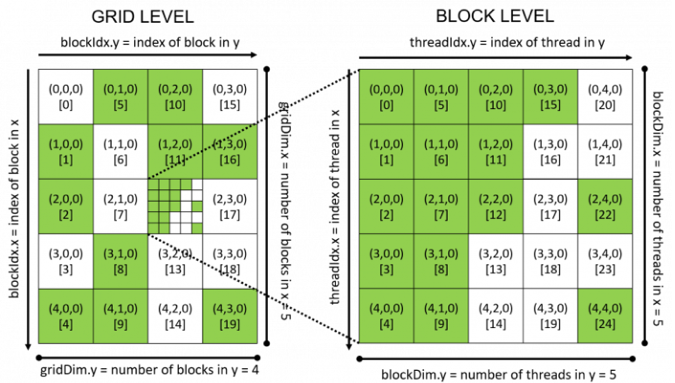
\includegraphics[scale=.8]{repGrid}
        \caption{Representación de los componentes de un grid\cite{CUDAP}.}
        \label{fig:grid}
    \end{figure}

    Para obtener ambos datos se aplica el algoritmo \ref{lst:idgb}:
    
    \begin{lstlisting}[style=CStyle, frame=single,label=lst:idgb,  basicstyle=\ttfamily\footnotesize, caption=Transformación para obtener el id del thread y del block.] 
    id_block = blockIdx.y * gridDim.x + blockId.x
    
    id_thread = threadIdx.y * blockDim.x + threadIdx.x
    \end{lstlisting}
    
    \begin{figure}[ht]
      \centering
        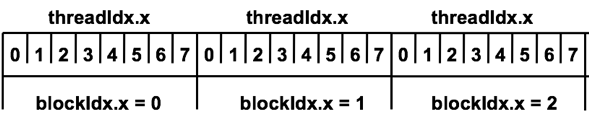
\includegraphics[scale=1]{idtb}
        \caption{Orden de threads y blocks dentro de un grid\cite{CUDAP}.}
        \label{fig:threadOrden}
    \end{figure}
    
    Existe una jerarquía memoria para las variables que se utilicen, la tabla \ref{tab:memoriaCUDA} muestra el lugar donde se almacenan y el alcance que tienen.
    
         \begin{table}[h!]
         \footnotesize
      \begin{center}
        \begin{tabular}{|m{4.6cm}|m{2.6cm}|m{2.6cm}|m{3cm}|}
         \hline
         \cellcolor{lightgray}\textbf{Declaración} & 
         \cellcolor{lightgray}\textbf{Memoria} &
         \cellcolor{lightgray}\textbf{Alcance} &
         \cellcolor{lightgray}\textbf{Tiempo de vida}\\ 
         \hline
        int x & registro & thread & thread\\ 
         \hline
        int arreglo\_x & local & thread & thread\\ 
         \hline
        \_\_shared\_\_ int shared\_x & shared & block & block\\ 
         \hline
        \_\_device\_\_ int global\_x & global & grid & aplicación\\ 
         \hline
           \end{tabular}
        \caption{Jerarquía de almacenamiento en device.}
        \label{tab:memoriaCUDA}
      \end{center}
    \end{table}
    
    \subsubsection{Perspectiva del hardware}
    
     \begin{table}[h!]
      \begin{center}
            \footnotesize
        \begin{tabular}{|m{3cm}|m{6cm}|}
         \hline
         \cellcolor{lightgray}\textbf{Warp} & Agrupación de threads que ejecutan la misma instrucción. \\ 
         \hline
          \cellcolor{lightgray}\textbf{Thread Block (TB)} & Varios warps constituyen un TB.\\ 
         \hline  
         \cellcolor{lightgray}\textbf{Streaming Multiprocessor (SM)} & Las unidades que ejecutan los arreglos de TB.\\ 
         \hline
         \cellcolor{lightgray}\textbf{GPU} & Varias SM forman una GPU.\\ 
         \hline
           \end{tabular}
        \caption{Componentes de CUDA para el hardware.}
        \label{tab:CUDAcompHW}
      \end{center}
    \end{table}
    
    Cada modelo de tarjeta gráfica contiene una cantidad variable de SM dependiendo de su tamaño y/o propósito. Cada uno puede ejecutar un número limitado de TB en concurrente. 
    Cada vez que un SM ejecuta un TB, cada uno de sus Threads se ejecuta al mismo tiempo, por lo tanto, para liberar los recursos ocupados y darle la oportunidad a un nuevo kernel de la cola de ejecución, es fundamental que todos los hilos de ese TB concluyan completamente su ejecución \cite{CuLect2}.
    \newline
    
    Un warp es la entidad mínima ejecutable dentro de la GPU y es un conjunto de 32 threads dentro de un TB, por lo que todos los hilos en su interior ejecutan la misma instrucción, y son seleccionados serialmente por el SM que los ejecutará. \cite{WarpLvl}
Una vez que se lanza un TB en un SM, todos los warps permanecen en ejecución hasta que todos sus threads completen su ejecución. Por lo que un TB nuevo no puede iniciarse dentro de un SM hasta que no haya un número suficiente de registros libres para que todos los warps de un TB puedan iniciar su ejecución.
    

    \subsection{Arquitectura Pascal}\label{secc:arqPas}

    La principal ventaja de la arquitectura Pascal está en su construcción ya que está implementada con transistores FinFET\cite{PasGPU}, los cuales al ser de un tamaño de 16 nanómetros, permiten tener un tamaño reducido, proporcionar un rendimiento alto y obtener una gran eficiencia energética. Dicha combinación la hacen ideal para ser implementada en dispositivos embebidos que requieran ejecutar tareas híbridas.
    \newline
   
   En esta arquitectura se implementaron dos cambios significativos que ayudan a mejorar el rendimiento de los sistemas. La primera la encontramos en la memoria unificada, la cual proporciona un único espacio de direcciones virtuales para la memoria de el CPU y GPU, permitiendo la migración transparente de datos entre los espacios de direcciones virtuales completos tanto de la tarjeta gráfica como del procesador. Esto simplifica la programación en GPUs y su portabilidad ya que, como programador, no es necesario el  preocuparse por administrar el intercambio de datos entre dos sistemas de memoria virtual diferentes\cite{WPNV}.
    \newline
   
     En la figura \ref{fig:direcMem} podemos observar tres tipos de código: el central es el código original que se ejecuta normalmente en un CPU. A la izquierda tenemos su versión en CUDA, y a la derecha se puede observar la versión en CUDA con memoria unificada. Con ello se puede observar que se ahorra mucho espacio de código para el manejo de la memoria entre CPU y GPU.
       \newline
       
  \begin{figure}[ht]
      \centering
        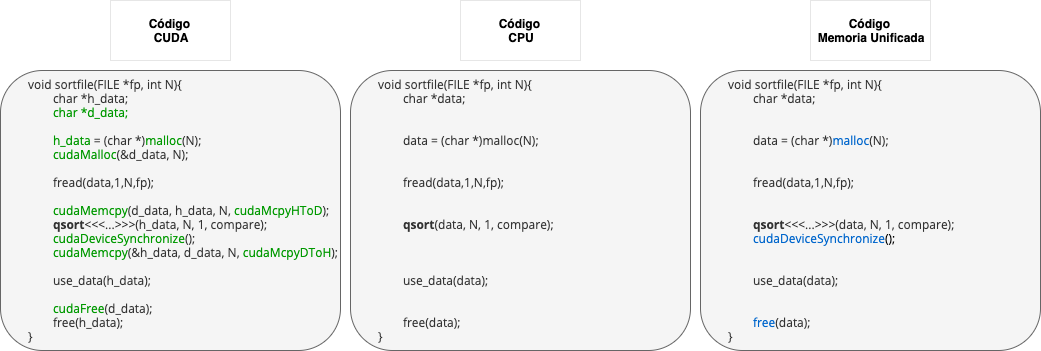
\includegraphics[scale=.45]{direcMem}
        \caption{Comparación de directivas para manejo de memoria.}
        \label{fig:direcMem}
    \end{figure}
     
    La segunda incorporación es la implementación de operaciones atómicas de memoria. Estas son frecuentemente usadas en el cómputo de alto rendimiento ya que permiten que los hilos concurrentemente lean, escriban y modifiquen variables compartidas sobre la memoria unificada.
     
    %Asignar memoria unificada es tan simple como reemplazar llamadas a malloc o cudaMalloc con llamadas a cudaMallocManaged\cite{}.
     
   % \subsubsection{Computación preemptive}
    %Permite que las tareas de cómputo se reemplacen con granularidad a nivel de instrucción, en lugar de bloque de subprocesos, evitando el funcionamiento prolongado de aplicaciones que monopolizan el sistema y no dejan ejecutar terceras tareas\cite{WPNV}. Obteniendo así, que las tareas puedan ejecutarse todo el tiempo que requieran ya sea para procesar grandes volúmenes de datos o qué esperen a que ocurran varias condiciones, mientras otras aplicaciones son computadas concurrentemente.

    %\subsubsection{Balanceo de carga dinámico}
    %La arquitectura Pascal introdujo el soporte para balanceo de carga dinámico \cite{AnPasc},  ayudando a la aceleración del cómputo de tareas asíncronas.
     %   \vspace{0.3cm}
        
    %En versiones anteriores de las tarjetas, la asignación de recursos en las colas de cálculos y de gráficos debía decidirse antes de la ejecución, por lo que, una vez que se lanzaba la tarea, no era posible reasignarla sobre la marcha. Un problema añadido que existía era, que, si una de las colas se quedaba sin trabajo antes que la otra no podía iniciar un nuevo trabajo hasta que ambas colas terminen completamente\cite{PasAna}.
    
   % \subsubsection{Operaciones atómicas} 
    %Las operaciones atómicas de memoria frecuentemente son importantes el cómputo de alto rendimiento ya que permiten que los hilos concurrentemente lean, escriban y modifiquen variables compartidas. La arquitectura Pascal nos permite realizar estas operaciones pero ahora con la ventaja de trabajar sobre memoria unificada.

    \subsection{GPGPU}
    
    Mientras que las GPU actuales ofrecen una gran potencia de procesamiento, a menudo es difícil aprovecharla. Por ello se han realizado esfuerzos que incluyen nuevos modelos de procesamiento con varios grados de paralelismo.
    \newline
   
    El cómputo  de propósito general en unidades de procesamiento de gráficos o GPGPU es utilizado para acelerar el procesamiento realizado tradicionalmente por el CPU únicamente, donde la GPU actúa como un coprocesador que puede aumentar la velocidad del trabajo \cite{GpuCpu}.
    
     \begin{figure}[ht]
      \centering
        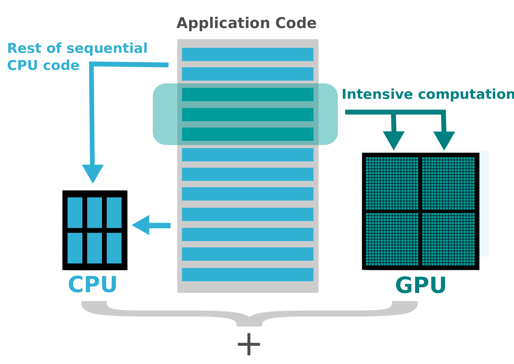
\includegraphics[scale=0.9]{gpgpu}
        \caption{Aceleración de programas en GPU\cite{gpgpu}.}
        \label{fig:gpgpu}
    \end{figure}
                
   \vspace{0.3cm}
   
    La unificación de los espacios de memoria facilita el GPGPU ya que no hay necesidad de transferencias explícitas de memoria entre el host y el dispositivo.
    
     %----------------------------------------------------------------------
    %SISTEMAS EMBEBIDOS
    \section{Sistemas embebidos}

    Un sistema embebido es un sistema de cómputo diseñado para realizar tareas dedicadas, su mayor reto es realizar tareas específicas donde la mayoría de ellas tengan requerimientos de tiempo real \cite{LimPree}.

    \subsection{Sistemas embebidos heterogéneos} \label{sec:seh}
    %
    \vspace{0.3cm}
    En los últimos años, los sistemas embebidos han ido demandando nuevas características debido a su rápida adopción en el mercado. Con lo que surge el desarrollo de sistemas embebidos heterogéneos, dónde está contemplado realizar una gran cantidad de cómputo pero con eficiencia tanto energética como espacial.
    \vspace{0.3cm}

    Actualmente la empresa NVIDIA tiene en su catálogo sistemas embebidos heterogéneos con un gran soporte y bibliotecas para el cómputo de alto rendimiento. Dichos sistemas cuentan con la arquitectura Pascal de última generación \cite{GPUArt}, la cual permite compartir memoria entre CPU y GPU.
               
   \vspace{0.3cm}
   
    % Framework
    Debido a que la mayoría de las GPU en sistemas embebidos no son de naturaleza preemptive, es importante programar los recursos de GPU de manera eficiente en múltiples tareas \cite{TX2I} ya sea de planificación o memoria, lo que permite pensar en un framework que ayude a la administración de sus características. 
    
 \section{Material de trabajo}
 
Para realizar la presente tesis, se tuvo acceso al sistema embebido heterogéneo NVIDIA Jetson TX2, en el cual se realizaron algunas pruebas para la familiarización con este tipo de dispositivos, así como la programación en tarjetas gráficas.
            
   \vspace{0.3cm}
   
En la figura \ref{fig:arqutecturaTX2} se muestra diagrama de bloques de la arquitectura del sistema Jetson TX2.

      \begin{figure}[ht]
      \centering
        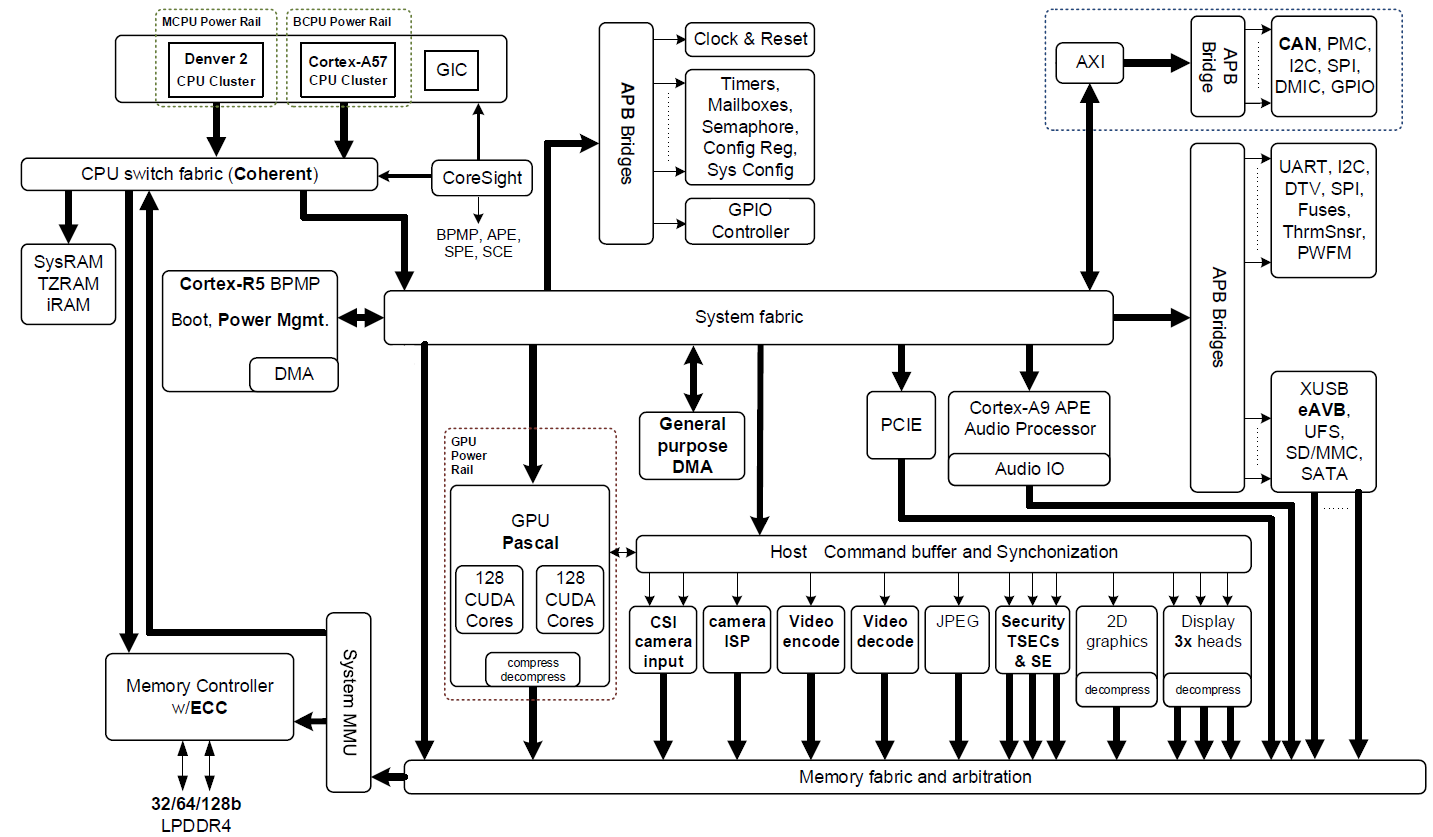
\includegraphics[scale=.44]{arqutecturaTX2}
        \caption{Diagrama de la arquitectura del sistema Jetson TX2\cite{ArqTX2}.}
        \label{fig:arqutecturaTX2}
    \end{figure}

 \subsection{Jetson TX2}
 
    Las especificaciones del sistema se están descritas en la tabla \ref{tab:jetson}.

    \begin{table}[h!]
      \begin{center}
            \small
        \begin{tabular}{|m{3cm}|m{5.5cm}|m{6.5cm}|}
         \hline
        \cellcolor{lightgray}\textbf{Elemento} & \cellcolor{lightgray} \textbf{Componentes} & \cellcolor{lightgray} \textbf{Descripción}\\ 
         \hline
         \textbf{Arquitectura} & NVIDIA Pascal GPU & 256 núcleos Optimizados para un mejor rendimiento en sistemas embebidos.\\
         \hline
         \textbf{CPU} & Dual-Core Denver 2 64-bit CPUs + Quad-Core A57 Complex & Contiene dos clústers de procesamiento, el Denver 2 de 64 bits que se utiliza para tareas pesadas o de un sólo thread; y el ARMv8 Cortex-A57 Complex que actúa en tareas multi-thread y en cargas ligeras.\\
         \hline
         \textbf{Memoria} & 8 GB L128 bit DDR4 Memory & DRAM de 128 bits que da soporte con un gran ancho de banda para una interfaz LPDDR4.  \\
          \hline
    	\textbf{Almacenamiento} & 32 GB eMMC 5.1 Flash Storage & Integrada en el módulo.\\
         \hline
    	\textbf{Conectividad} & 802.11ac Wi-Fi and Bluetooth-Enabled Devices & \\
         \hline
   	 \textbf{Ethernet} &10/100/1000 BASE-T Ethernet & \\
	  \hline
   	 \textbf{Procesador de señales} &1.4Gpix/s Advanced image signal processing & Acelerador por hardware para captura de video y de imágenes.\\
	 &Audio Processing Engine & Subsistema que permite el completo soporte de audio multicanal por las diversas interfaces.\\
	 \hline
   	 \textbf{Video} & Codificador avanzado de video HD & Permite la grabación de video ultra-high-definition a 60 fps, soporta los estándares H.265 and H.264 BP/MP/HP/MVC, VP9 y VP8. \\
	  & Decodificador avanzado de video HD & Reproducciónde video ultra-high-definition a 60 fps con pixeles de 12 bits, soporta los estándares H.265, H.264, VP9, VP8 VC-1, MPEG-2, y MPEG-4. \\
         \hline
   	 \textbf{Controlador de la pantalla} &eDP/DP/HDMI Multimodal & Realiza un almacenamiento multilínea de pixeles, lo que permite mayor eficiencia de memoria al momento de aplicar operaciones de escalamiento o de búsqueda de pixeles. Permite la reducción del ancho de banda en aplicaciones móviles.\\
         \hline
        \end{tabular}
        \caption{Especificaciones del sistema Jetson TX2\cite{jtx2dk}.}
        \label{tab:jetson}
      \end{center}
    \end{table}
       
   Algunas de las tareas realizadas con el dispositivo incluyen desde la familiarización hasta la puesta a punto, como son:
   \begin{itemize}
    \item Instalación del Sistema Operativo Ubuntu 18 para procesadores ARM.
     \item Instalación de CUDA manager.
     \item Actualización de bibliotecas compatibles.
     \item Configuración de área local y conexión a través de computadora remota.
      \item Investigación e implementación de ejercicios de GPGPU.
       \item Realización y modificación de ejercicios para la familiarización con la arquitectura Pascal, estructura de la tarjeta y su memoria.
    \end{itemize}   
   

%%Capítulo 3 trabajo relacionado 
 \chapter{Trabajo Relacionado}
    \label{cha:TrabajoRelacionado}
   
  Durante la revisión de la literatura referida a este estado del arte, se encontró que existe muy poca bibliografía sobre el tema debido a que las empresas manufactureras de las tarjetas gráficas no liberan suficiente información al público en general, ya que sus diseños no están documentados o se describen a alto nivel que no revelan los detalles técnicos cruciales.
\newline

Se realizó un estudio en \cite{TX2-H} con base en la documentación y pruebas de caja negra sobre la arquitectura Pascal. Como caso de estudio utilizaron el sistema NVIDIA Jetson TX2, que es precisamente el que se tuvo disponible al realizar esta tesis.
%\newline

El estudio tiene como objetivo dar las pautas para realizar normas oficiales de seguridad a los sistemas embebidos heterogéneos y así poder certificar su uso en ambientes críticos. 
\newline

Cada GPU contiene un arreglo de Streaming Multiprocesor (SM) dependiendo del modelo o arquitectura, en donde cada SM puede procesar concurrentemente una misma cantidad de threads. Como ya se mencionó anteriormente, las empresas que producen el hardware no revelan mucho sobre las peculiaridades de cómo se realiza el reparto de recursos para ejecutar las peticiones. Únicamente sabemos que la GPU distribuye los blocks pendientes dentro de los SM en grupos de 32 threads, estos grupos son llamados warps. Un warp es una entidad planificable de un SM.
Un block puede ser asignado únicamente a un SM si este tiene suficientes recursos para recibirlo, si no, esperará hasta que pueda ser lanzado. El cómo realiza esta espera tampoco es revelado por las compañías.
\newline

El sistema Jetson TX2 cuenta con 2 SM, y cada uno con 128 cores que en conjunto pueden procesar concurrentemente 2048 threads\cite{SMJetson}, por lo que cada SM puede manejar un máximo de 64 warps.
\newline

Por ejemplo, en la tabla \ref{tab:asigUnKernelSM} se muestran diversos escenarios en los que se desea agregar kernels para procesar a la tarjeta gráfica.
\newline

  \begin{table}[h!]
      \begin{center}
            \scriptsize
        \begin{tabular}{|m{1.5cm}|m{1cm}|m{1cm}|m{1.5cm}|m{1.5cm}|m{1cm}|m{1cm}|m{1cm}|m{1cm}|m{1.5cm}|}
         \hline
         \cellcolor{lightgray}\textbf{Escenario} &
         \cellcolor{lightgray}\textbf{Kernel} & 
         \cellcolor{lightgray}\textbf{Blocks} &
         \cellcolor{lightgray}\textbf{Threads por block} &
         \cellcolor{lightgray}\textbf{Threads Totales} &
         \cellcolor{lightgray}\textbf{Blocks SM0} &
         \cellcolor{lightgray}\textbf{Warps SM0} &
         \cellcolor{lightgray}\textbf{Blocks SM1} &
         \cellcolor{lightgray}\textbf{Warps SM1} &
         \cellcolor{lightgray}\textbf{Threads utilizados}\\ 
         \hline
         A & K2 & 4 & 512 & 2048 & 4 & 64 & 0 & 0 & 2048\\ 
         \hline
         B & K1 & 16 & 265 & 4096 & 8 & 64 & 8 & 64 & 4096\\ 
         \hline
         C & K3 & 9 & 350 & 3150 & 5 & 55 & 4 & 44 & 3168\\ 
         \hline
           \end{tabular}
        \caption{Asignación de un solo kernel a los SM.}
        \label{tab:asigUnKernelSM}
      \end{center}
    \end{table}
    
    En el escenario \textbf{(A)} (ver figura \ref{fig:asigBlock}) tenemos el kernel \textbf{K2} con 4 blocks y cada uno de 512 threads. La primera condición para poder agregarlo recae en que la totalidad del kernel debe poder ejecutarse en concurrente en la tarjeta gráfica durante un  instante de tiempo. En este caso, recordemos que un SM tiene un máximo de 64 warps disponibles, y el kernel justamente está constituido por esa cantidad, por lo que el planificador de hardware de la tarjeta asigna secuencialmente los blocks a las localidades.
    \newline
    
    En el escenario \textbf{(B)} se agrega un kernel que comprende 16 blocks y cada uno consta de 256 threads por block. En este caso, al lanzarlo se utilizará la totalidad de los recursos de la GPU y los blocks se irán asignando secuencialmente empezando desde la primer localidad del \textbf{SM0} y así sucesivamente hasta que se terminen sus recursos. Cuando esto suceda, se continuará con las primeras localidades de \textbf{SM1} hasta terminar de lanzar todos los blocks del kernel. En caso de que existan recursos para colocar blocks de un kernel al final de \textbf{SM0} pero no los suficientes para colocarlo al inicio de \textbf{SM1}, el kernel no se podrá lanzar, y el planificador por hardware saltará la tarea y asignará otra que ocupe menos recursos.
    \newline
    
    \begin{figure}[ht]
      \centering
        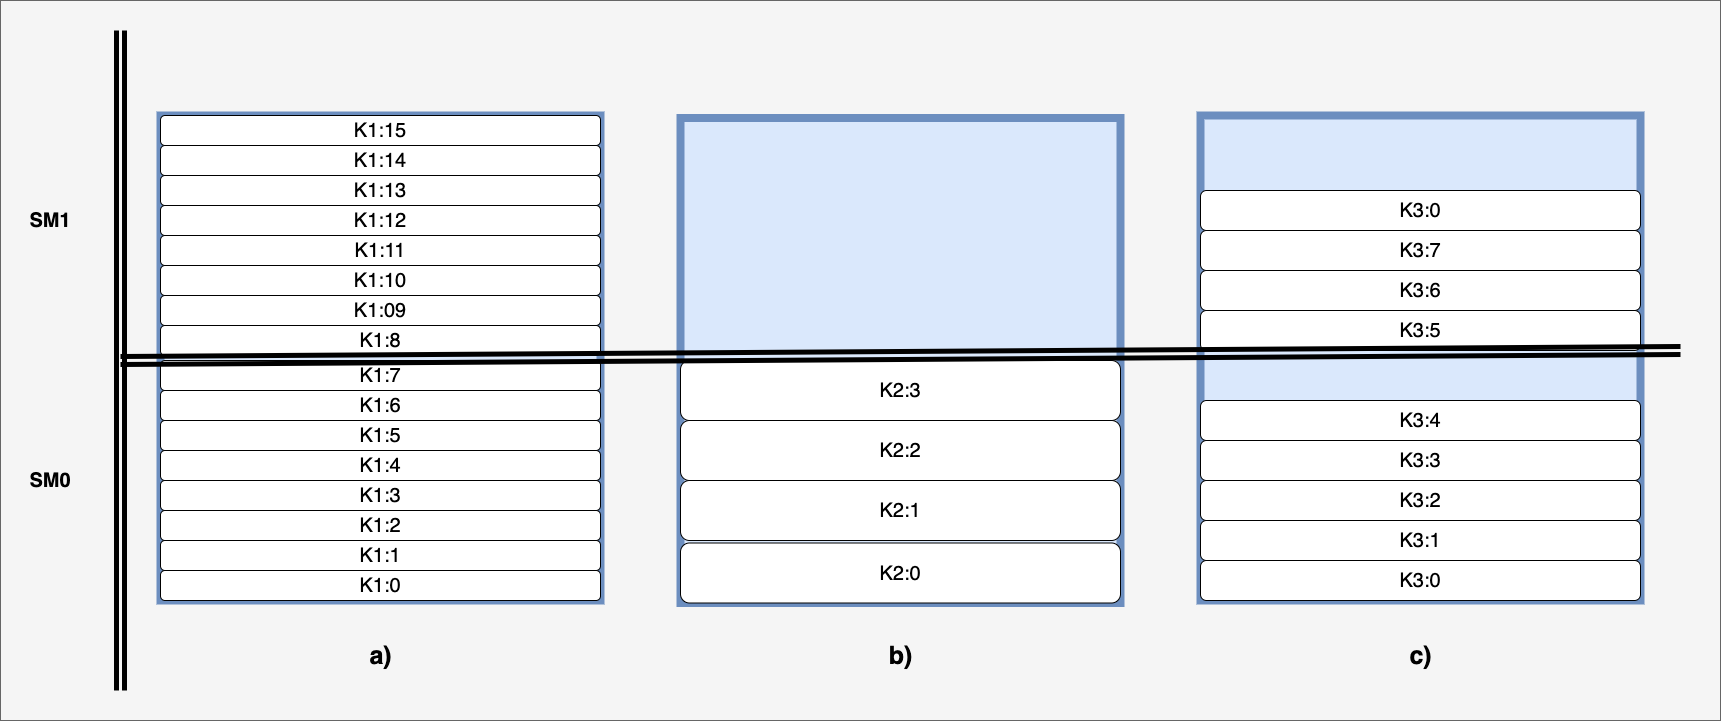
\includegraphics[scale=.275]{asigBlock}
        \caption{Diagrama de asignación de un kernel a los SM.}
        \label{fig:asigBlock}
    \end{figure}
    
    Finalmente, en el escenario \textbf{(C)} deberían ser 54.6 warps en el \textbf{SM0} utilizando 1750 threads, pero en realidad se utilizan 55 warps, con lo que el trabajo de 10 threads y 9 warps se desperdician. En el \textbf{SM1}, deberían ocuparse 43.75 warps, pero se usan 44, dejando 8 threads y 20 warps sin poderse utilizar.
    \newline
    
Habitualmente en sistemas GPGPU se requiere lanzar más de un kernel a la vez, en la tabla \ref{tab:asigVariosKernelsSM} se tienen 3 situaciones en las que esto podría ocurrir.
\newline

    \begin{table}[h!]
      \begin{center}
            \scriptsize
        \begin{tabular}{|m{1.5cm}|m{1cm}|m{1cm}|m{1cm}|m{1cm}|m{1cm}|m{1cm}|m{1cm}|m{1cm}|m{1cm}|m{1cm}|}
         \hline
         \cellcolor{lightgray}\textbf{Escenario} & 
         \cellcolor{lightgray}\textbf{Kernel} & 
         \cellcolor{lightgray}\textbf{Blocks} &
         \cellcolor{lightgray}\textbf{Threads por block} &
         \cellcolor{lightgray}\textbf{Threads por kernel} &
         \cellcolor{lightgray}\textbf{Threads en concurrente} &
         \cellcolor{lightgray}\textbf{Warps} &
         \cellcolor{lightgray}\textbf{Warps aportados a SM0} &
         \cellcolor{lightgray}\textbf{Warps SM0} &
         \cellcolor{lightgray}\textbf{Warps aportados a SM1} &
         \cellcolor{lightgray}\textbf{Warps SM1} \\ 
         \hline
         \multirow{2}{1cm}{D} & K1 & 3  & 512 & 1536 & \multirow{2}{1cm}{4096} & 48 & 48 & \multirow{2}{1cm}{64} & 0  & \multirow{2}{1cm}{64}\\ 
                              & K2 & 10 & 256 & 2560 &                         & 80 & 16 &                       & 64 & \\ 
         \hline \hline
        \multirow{3}{1cm}{E} & K1 & 1 & 1024 & 1024 & \multirow{3}{1cm}{2304} & 32 & 32 & \multirow{3}{1cm}{64} & 0  & \multirow{3}{1cm}{8}\\ 
                             & K2 & 1 & 768  & 768  &                         & 24 & 24 &                      & 0 & \\ 
                             & K3 & 2 & 256  & 512  &                         & 16 & 8 &                       & 8 & \\ 
         \hline \hline
        \multirow{3}{1cm}{F} & K1 & 1 & 768  & 768  & \multirow{3}{1cm}{3072} & 24 & 24 & \multirow{3}{1cm}{24} & 0  & \multirow{3}{1cm}{48}\\ 
                             & K2 & 1 & 1536 & 1536 &                         & 48 & 0  &                       & 48 & \\ 
                             & K3 & 1 & 768  & 768  &                         & 24 & 0  &                       & 0 & \\ 
         \hline
           \end{tabular}
        \caption{Asignación de varios kernels a los SM.}
        \label{tab:asigVariosKernelsSM}
      \end{center}
    \end{table}
    
    En el escenario \textbf{(D)} (ver figura \ref{fig:KernelSM}) se desea asignar dos kernels, uno de 3 blocks y otro de 10. Recordemos que la restricción es que un kernel sólo puede ser asignado si existen suficientes recursos para warps en secuencia. La primer tarea utiliza 48 warps, y la segunda 80, por lo que en \textbf{SM0} podemos asignar los 48 warps del primer kernel más 16 del segundo, y en el \textbf{SM1} colocamos los 64 restantes, ocupando así la totalidad de localidades de la GPU.
    \newline
    
    Continuando con el caso \textbf{(E)}, ahora tenemos 3 kernels, dos de un block con 1024 threads y otro con 768, respectivamente y uno con 2 blocks de 256 threads, en conjunto ocupan 72 warps en total, por lo que podemos asignar los 32 warps del \textbf{K1} al \textbf{SM0}, justo después los 24 del \textbf{K2} y aún sobran 8 warps que sirven perfectamente para ejecutar la mitad de warps del \textbf{K3} y, como las localidades del inicio de \textbf{SM1} están disponibles, se sigue con la asignación de los 8 restantes.
    \newline
    
    El escenario \textbf{(F)} presenta un caso en que se tienen 3 kernels que en conjunto representan 3072 threads, lo que nos hace pensar que muy bien pueden ser ejecutados en concurrente dentro de la GPU, pero el orden de lanzamiento influye de primera mano en la repartición de los recursos. Primero se lanza el kernel \textbf{K1} que constituye 24 warps, después se recibe la petición de  \textbf{K2} con 48, pero como no es posible asignarlo en el \textbf{SM0}, se le asignan las localidades de \textbf{SM1}. Finalmente, desea despachar a \textbf{K3} con 24 warps, pero como la asignación de recursos se realiza de forma secuencial, se empieza a preguntar justo en la siguiente localidad de la última asignada, con lo que ya no es posible lanzar esa tarea, y se deberá esperar a que terminen su ejecución las tareas actuales. Aunque en el \textbf{SM0} sobran recursos que bien podrían aprovecharse, la documentación actual no permite realizarlo, por ello se recurrió a una solución en la sección \ref{secc:balanceador}.
    \newline
    
    \begin{figure}[ht]
      \centering
        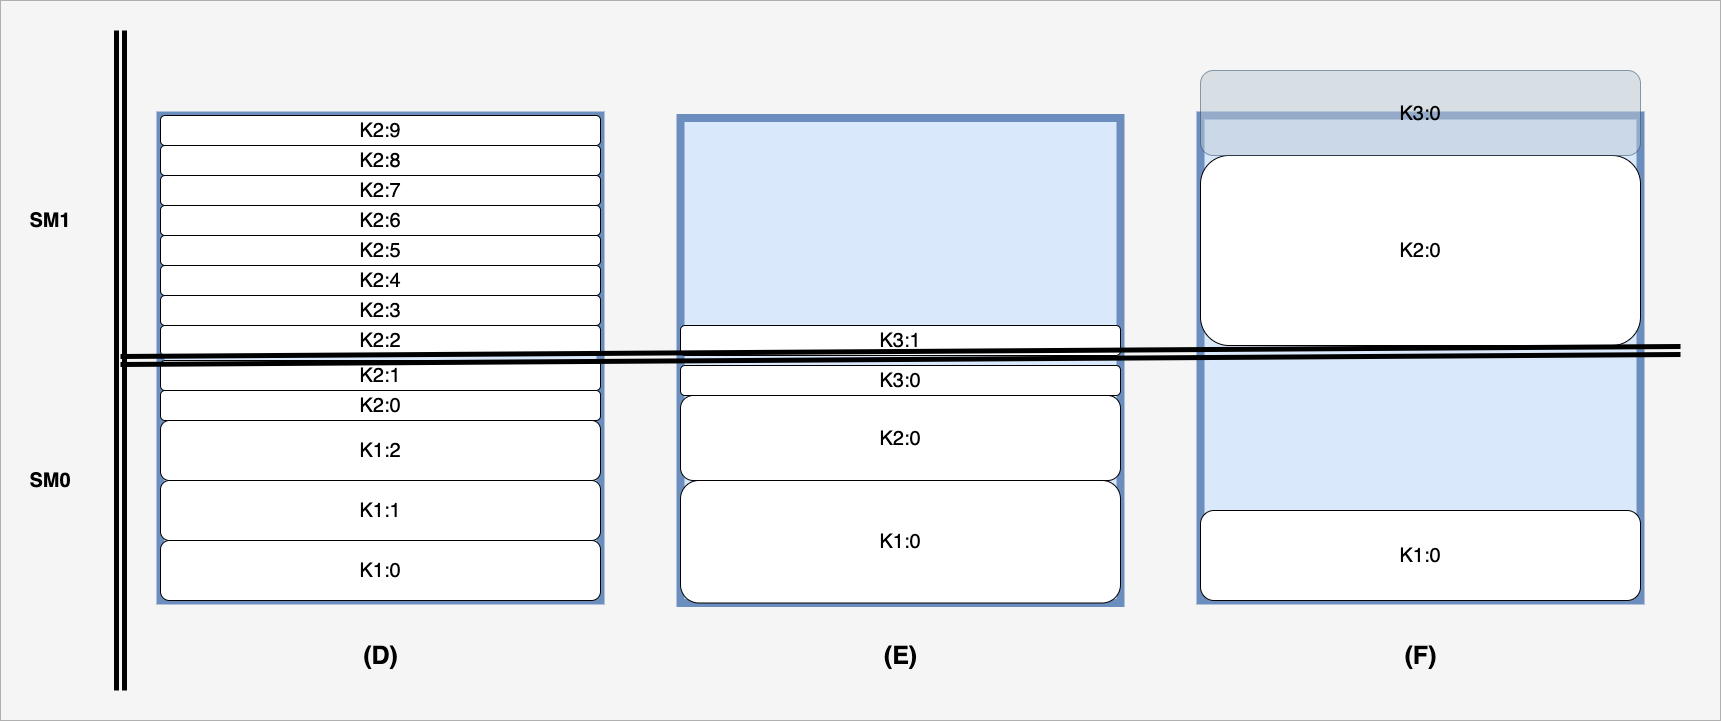
\includegraphics[scale=.275]{KernelSM}
        \caption{Diagrama de asignación de varios kernels a los SM.}
        \label{fig:KernelSM}
    \end{figure}

   Ahora bien, teniendo una referencia por medio de pruebas de software, se puede conocer un poco sobre el funcionamiento de la asignación de kernel a la tarjeta gráfica. Se puede afirmar que es posible gestionar las peticiones de recursos a la GPU, y el programador debe cuidar que tamaño de los bloques de threads sean múltiplos de 32 o al menos potencia de 2 para optimizar los recursos de la tarjeta gráfica y así ejecutar la mayor cantidad posible de tareas concurrentemente.
\newline
    
%Clasificación
Para poder utilizar varias aplicaciones con sistemas en tiempo real complejos es necesario utilizar técnicas de implementación preemptive\cite{RGEM}. Algunos trabajos han utilizado estas técnicas para mejorar el rendimiento de las aplicaciones gráficas en tiempo real, principalmente para la reconstrucción de imágenes en 3D y la detección de rostros\cite{DynSche}.
\newline

La clasificación de la planificación de tareas preemptive esta compuesta de diversos tipos dependiendo de sus técnicas de implementación, cómo se describe en la sección \ref{claspree}. 
%Basado en hardware
Las soluciones basadas en hardware son costosas, ya que debemos desarrollar y construir un dispositivo que auxilie con el cambio de contexto. Por ejemplo, en el artículo \cite{18} se utilizan extensiones de hardware a modo de registros que almacenan el contexto y, en general, las direcciones de memoria que contienen la información necesaria para la restauración de la ejecución de un kernel. 

\vspace{0.3cm}

Se ha propuesto\cite{20} la utilización de extensiones de hardware mediante el intercambio equitativo de recursos entre los núcleos de procesamiento, realizando un cambio de contexto al aplicar el modo preemptive en el espacio de procesamiento. En lugar de intercambiar el contexto de todo el grid, se pretende intercambiar suficientes TB de un kernel en ejecución para que haya suficientes recursos disponibles para despachar la nueva tarea. 

\vspace{0.3cm}

Otra solución la observamos en \cite{8}, donde se desarrolló un compilador que emplea una extensión de hardware para reducir la latencia al implementar el modo preemptive. El compilador inserta puntos preemptive utilizando un análisis del ciclo de vida de los registros. Se utiliza una lógica de compresión-descompresión para disminuir el tamaño del contexto de una tarea. Es decir, cuando el valor almacenado en un determinado registro es siempre igual a lo largo de la ejecución de los TB de un kernel, sólo se guardará un valor durante el cambio de contexto.
\newline
%Para aquellas basadas en software, 

%tenemos por una parte las que parten el kernel como
%Basado en Software : Partición de kernel
El articulo \cite{GPES} implementa \textit{GPES}, una serie de funciones para realizar particiones de kernel y de datos, esto realizando subkernels y dividiendo las transacciones de datos en fragmentos. 
Específicamente, se presenta una técnica de reescritura binaria para reconfigurar de manera transparente el código de los kernel. Mientras que para los kernel un poco más complejos, se desarrolló una técnica de transformación fuente a fuente que compila el código del kernel transformado en binarios CUDA. La prioridad de las tareas esta dada por colas de ejecución. GPES modifica el API de CUDA utilizando las bibliotecas de  \textit{openCUDA} para reconfigurar el código binario de los kernels, esto lo realiza obteniendo un máximo de blocks que se pueden ejecutar por quantum. Para llevarlo a cabo se realiza una transformación fuente a fuente apoyándose en la partición de la transferencia de datos.
\newline

En el artículo \cite{RTFG} se propone un framework de planificación que parte los kernels de la GPU y genera secuencias de lanzamiento en subkernels dinámicamente para entrar en el modo preemptive con la implementación de un divisor de carga de trabajo y de un planificador de tareas. 
Utiliza un divisor de carga de trabajo que fracciona el kernel GPU en múltiples subkernels en tiempo de ejecución para implementar el modo preemptive. Dependiendo del estado actual del sistema y de la prioridad, el divisor de carga de trabajo decide el número y el tamaño de cada subkernel. 

También cuenta con un generador de ejecución planificada, el cual, dependiendo del estado actual de uso de los recursos del sistema y del plazo límite de la tarea, lanza una secuencia de tareas para maximizar el número de aplicaciones cercanas a su plazo vencido.	
\newline

El trabajo \cite{Effisha} describe el framework EffiSha que se basa en un entorno de scripts que permite convertir los kernels automáticamente a modo preemptive. Esta solución consta de componentes que funcionan tanto en tiempo de compilación como en el de ejecución. 
En tiempo de compilación realiza una transformación de fuente a fuente que transforma un programa para la gestión y planificación oportuna de su tiempo de ejecución.
En el código del CPU, reemplaza las llamadas a función de la GPU con las del API de EffiSha, así modifica los kernel GPU para que puedan acelerar el cambio o drenado de contexto durante el tiempo de ejecución. También se analizan e identifican aquellos datos que no se volverán a utilizar después de la restauración de contexto, con lo que ahorra el tiempo de las transacciones de memoria innecesarias.
%\newline

La fase de ejecución consiste en un daemon en el lado del CPU y un proxy de éste en el lado de la GPU. Dicho daemon gestiona el momento en que los kernel deben comenzar, reanudarse o detenerse en la GPU, y dependiendo de la acción se notifica al proceso del CPU que fue lanzado.
%\newline

Como muestran los resultados del trabajo, esta solución funciona bien para kernels con ejecución pequeña porque al tener en el sistema aquellos que salen de la media, la granularidad del TB limita el retraso mínimo preemptive que se puede lograr, resultando muy seguramente en plazos vencidos.
%\newline
 
 Es importante mencionar que el artículo \cite{RGEM} es el primer trabajo que genera un framework para utilizar tareas en tiempo real en tarjetas gráficas. 
 Este trabajo entra dentro de la categoría de colas masivas en paralelo, ya que se basa en la partición en fragmentos de memoria a procesar y cada fragmento es agregado a una cola de procesamiento para ser ejecutado. Su solución es dividir las transacciones de copiado de memoria en varios fragmentos para insertar puntos preemptive. 
 Esto también garantiza que sólo las tareas de mayor prioridad se ejecuten en la GPU en cualquier momento, y así evitar interferencias de rendimiento causadas por lanzamientos concurrentes.

	La primera característica de este framework es que se basa en transacciones de datos preemptive, por lo que los tiempos de bloqueo están limitados para copiar cada fragmento de dato. La segunda característica es que permite lanzar los kernels de diferentes tareas una por una basadas en su prioridad, lo que evita que las tareas con alta prioridad sean interferidas por la carga simultánea de trabajo una vez iniciadas. 
	Sin embargo el lanzamiento del kernel puede bloquearse al haber un kernel de menor prioridad lanzado anteriormente, esto debido al probable alto uso de memoria global.
\newline

El artículo \cite{PreeK} se basa en preguntar continuamente si ha terminado el quantum de una tarea, en caso afirmativo detiene la ejecución e ingresa la siguiente. Las tareas son almacenadas en una cola, por lo que todas tienen la misma prioridad durante la vida del sistema. Se propone un esquema de puntos de control donde se almacena el estado de un kernel en ejecución en la memoria del CPU en vez de la GPU. Para ello, se apoya de una estructura donde se almacena el contexto completo de la tarea. 
Para disminuir la latencia entre cada punto preemptive, se le avisa al framework que se debe tener preparada la estructura de seguridad con directivas \textit{pragma}, antes y después de la ejecución parcial de un kernel. Para ello fue necesario implementar un analizador sintáctico que ayudara al compilador a verificar las modificaciones del código.
\newline

El artículo \cite{IntraNode} propone la creación del framework schedGPU, el cual utiliza el administrador de trabajo Slurm para planificar las tareas. Este framework administra las múltiples solicitudes para acceder a la GPU de forma segura al garantizar que no se produzcan sobrecargas de memoria durante su ejecución. 
Este acceso es controlado mediante bloqueos de archivos, señales del sistema y exclusión mutua.
\newline

SchedGPU utiliza el patrón de diseño cliente-servidor ya que toma cada tarea que busca ser lanzada en la GPU como un cliente que está solicitando memoria a un servidor centralizado (en el mismo nodo), el cual permite que se ejecute si hay suficiente memoria; o en caso contrario, la bloquea hasta que se encuentre memoria necesaria para su funcionamiento. 
El servidor crea un nuevo hilo para cada cliente y mantiene una visión global de la memoria utilizada por todos los clientes a través de la biblioteca de administración de NVIDIA (\textit{NVML})\cite{TORQUE}, esto para evitar la creación de un nuevo contexto que consuma memoria.

La tarea es modificada únicamente al llamar  de manera explícita las funciones de la biblioteca del cliente para previamente asignar la memoria requerida al GPU. Esto acarrea una gran desventaja al considerar tareas donde no siempre es posible conocer la memoria requerida total de GPU, ya que la memoria de la GPU se asigna en tiempo de ejecución. 
En el caso en que dos o más tareas se ejecuten al mismo tiempo y ambas aumenten gradualmente, el uso de la memoria de la GPU se puede llegar a utilizar completamente, con lo que podrán requerir más tiempo para completar la ejecución o directamente lanzar un error de desbordamiento de memoria en tiempo de ejecución.
\newline	
	%Al utilizar schedGPU se encontró que el promedio de la aceleración aumenta 10 veces, comparado con no utilizar el framework. Sin embargo, el promedio de utilización de la memoria también incrementó de 5 a 12 veces.
	
	%Administración dinámica de los núcleos de procesamiento.
	El artículo \cite{Pridriven} presenta una técnica para la ejecución en GPUs llamada \textit{"Planificación de recursos compartidos con reserva de presupuesto"} o por sus siglas en inglés \textit{BR-SRS}, la cual limita el número de núcleos de procesamiento de una GPU para una tarea basándose en su prioridad, esto lo realiza modificando las bibliotecas de  \textit{OpenGL-ES}. 
	Así se previene que una tarea que se encuentra en segundo plano retrase a otra que se encuentra en ejecución, también se minimiza la sobrecarga de planificación al invocarse solamente dos veces, en el inicio de la tarea y en su finalización.
%\newline
%Planificación por prioridad

El único trabajo que utiliza algoritmos para la planificación de tareas en tiempo real, hasta el momento de la revisión del estado del arte es GPUart \cite{GPUArt}. 
Permite la implementación preemptive dentro de los TB y cada uno de estos subkernels se pueden planificar bajo las políticas de Earliest Deadline First (EDF) y de aquellos algoritmos que mantengan la prioridad de las tareas fijas.

GPUart se centra en las GPUs integradas, es decir, en las GPU que se colocan en la misma placa que el CPU. Esto porque permiten tener cero copias de memoria, lo que hace que las transferencias entre CPU y GPU sean nulas al compartir físicamente una memoria común. 
Por ello, GPUart no considera la planificación de transferencias de memoria a través del acceso directo a memoria (DMA).
\newline

A continuación se muestra la tabla \ref{tab:clasifTrabajos} con los trabajos relacionados y la clasificación en la que entran dependiendo de las características con que se ejecutan, así como su referencia en el bibliografía.
 	
  \begin{table}[h!]
      \begin{center}
            \footnotesize
        \begin{tabular}{|m{.6cm}|m{6cm}|m{2.7cm}|m{2.6cm}|m{2.6cm}|}
         \hline
        \cellcolor{lightgray}\textbf{Ref.} & \cellcolor{lightgray} \textbf{Artículo} & \cellcolor{lightgray} \textbf{Clasificación por implementación} & \cellcolor{lightgray} \textbf{Clasificación por planificación} & \cellcolor{lightgray} \textbf{Clasificación por Modificación}  \\ 
         \hline
          \textbf{\cite{18}} & \textbf{Enabling preemptive multiprogramming on GPUs} &  Basado en Hardware: Añade registros para almacenar contexto & Colas masivas en paralelo & Modificación del API\\
           \hline
          \textbf{\cite{20}} & \textbf{Simultaneous Multikernel GPU: Multi-tasking throughput processors via fine-grained sharing} &  Basado en Hardware: Selector de núcleos de procesamiento & Administración dinámica de los núcleos de procesamiento & Modificación del API\\
           \hline
           \textbf{\cite{8}} & \textbf{Enabling Efficient Preemption for SIMT Architectures with Lightweight Context Switching} &  Basado en Hardware: Analizador del ciclo de vida de registros & Administración dinámica de memora &Modificación del API\\
           \hline
             \textbf{\cite{GPES}} & \textbf{GPES: A preemptive execution system for gpgpu computing} & Basado en Software: Partición de kernel & Administración dinámica de memora &Modificación del API\\
           \hline
             \textbf{\cite{RTFG}} & \textbf{Run-Time Scheduling Framework for Event-Driven Applications on a GPU-Based Embedded System*} & Basado en Software: Partición en tareas & Administración dinámica de la memoria & Modificación del código fuente\\
            \hline
            \textbf{\cite{Effisha}} & \textbf{Effisha: A software framework for enabling efficient preemptive scheduling of GPU} & Basado en Software: Entorno de scripts & Colas masivas en paralelo & Modificación del API y código fuente\\
            \hline
          \textbf{\cite{RGEM}} & \textbf{RGEM: A Responsive GPGPU Execution Model for Runtime Engines} & Basado en Software: Partición de kernel & Colas masivas en paralelo & Modificación de código fuente\\
           \hline
           \textbf{\cite{PreeK}} & \textbf{Preemption of a CUDA Kernel Function} & Basado en Software: Partición de kernel & Colas masivas en paralelo & Modificación del API\\
            \hline
            \textbf{\cite{IntraNode}} & \textbf{Intra-Node Memory Safe GPU Co-Scheduling} &Basado en Software: Partición de kernel & Administración dinámica de la memoria & Modificación del API\\
            \hline
            \textbf{\cite{Pridriven}} & \textbf{Priority-driven spatial resource sharing scheduling for embedded graphics processing units} & Basado en Software: Partición en tareas &Administración dinámica de los núcleos de procesamiento & Modificación del API\\
            \hline
          \textbf{\cite{GPUArt}} & \textbf{GpuArt: An application-based limited preemptive gpu real-time scheduler for embedded systems*} & Basado en Software: Partición de kernel & Planificación por prioridad & Modificación de código fuente \\
            \hline
          
                \end{tabular}
        \caption{Matriz de clasificación de trabajos relacionados.}
        \label{tab:clasifTrabajos}
      \end{center}
      \begin{tablenotes}
      \small
      \item \textit{* Artículos que fueron diseñados específicamente para sistemas embebidos.}
    \end{tablenotes}
    \end{table}
    
    
    \begin{comment}
\section{Resumen}
%----------------------------------------------------------------------
    %RESUMEN
Este capítulo presenta los trabajos relacionados con el tema de esta tesis, se analizan 
\begin{itemize}
	\item Planificación de EDF preemptive limitado de sistemas con tareas esporádicas
	 (\textit{Limited Preemption EDF Scheduling of Sporadic Task Systems});
	 %
	 \item Planificación de recursos espaciales compartidos con prioridad para unidades de gráficos embebidos 
	 (\textit{Priority-driven spatial resource sharing scheduling for embedded graphics processing units});
    	 %
	\item Framework para planificación en tiempo de ejecución de aplicaciones con manejo de eventos en sistemas embebidos basados en GPU 
	(\textit{Run-Time Scheduling Framework for Event-Driven Applications on a GPU-Based Embedded System});
		%
	\item Sobre planificación dinámica para la GPU, sus aplicaciones en computación gráfica y más
	(\textit{On Dynamic Scheduling for the GPU and its Applications in Computer Graphics and Beyond}); y
	%
	\item REGM: Un modelo de ejecución GPGPU responsivo para soluciones en tiempo de ejecución
	(\textit{REGM: A Responsive GPGPU Execution Model for Runtime Engines});
	%
    	\item Planificación conjunta con GPU y aseguramiento de la memoria intra-nodo 
	(\textit{Intra-Node Memory Safe GPU Co-Scheduling});
 \end{itemize}
%----------------------------------------------------------------------
\end{comment}
%\vspace{0.3cm}
%Cada sección presenta lo propuesto en el trabajo relacionado, donde se describe el problema, los objetivos y la solución a éste. Brevemente se describe la solución propuesta con los resultados obtenidos y por último se presentan las conclusiones del trabajo.





%The earliest deadline first (EDF) scheduling algorithm is a typical representative of the dynamic priority scheduling algorithm. However, once the system is overloaded, the deadline miss rate increases and the scheduling performance deteriorates sharply, which causes a reduction in system resource utilization.

%En la práctica, ambas visiones de planificación, tanto preemptive, como non-preemptive, tienen ventajas y desventajas comparadas entre sí, por lo que ninguna es superior a la otra. Pero el patrón encontrado es que es necesario en pensar en un Framework qué brinde ayuda a la ejecución de tareas y que permita guardar el contexto en un tiempo específico. 

%Hoy en día, los sistemas embebidos basados en GPU han empezado a considerarse esenciales debido a su alta programabilidad y capacidad de desarrollo con técnicas de alto rendimiento, sumado a su bajo consumo energético. Estos exigen una mayor potencia de cálculo y deben responder a muchos eventos, por lo que se han buscado estrategias, y ahora comparten la memoria entre el CPU y la GPU, lo que resulta en una latencia muy cercana a cero.

%Se han propuesto diversos frameworks de última generación para planificación de tareas para aprovechar el rendimiento de los sistemas embebidos basados en GPU y su bajo consumo de energía.

%%%%%

%En este capítulo se presenta el resumen de tres trabajos relacionados con la evaluación de los patrones de seguridad. El primer trabajo presenta una métrica de seguridad denominada SC la cual contabiliza el total de amenazas mitigadas por patrones de seguridad entre el total de amenazas. Una de las mejoras que propone es utilizar la aproximación \textit{Twin peaks} que produce una nueva arquitectura en cada ciclo contemplando los mismos casos de uso pero a mayor detalle.

%\vspace{0.3cm}

%El segundo trabajo presenta una metodología que consiste en medir qué extensión de una arquitectura está protegida con respecto a las amenazas de seguridad más relevantes. La metodología consiste en cuatro partes: 1) mapeo de las amenazas con los objetivos de seguridad, 2) clasificación de las amenazas de acuerdo a su severidad, 3) determinación de la protección ante una amenaza y 4) cálculo de la cobertura de seguridad. 

%\vspace{0.3cm}

%Por último, el tercer trabajo presenta una metodología que permite elegir los patrones de seguridad con respecto a los objetivos de seguridad y las métricas que evaluarán a los patrones. La metodología se divide en tres fases que son: 1) definición de los patrones de seguridad a partir de los objetivos de seguridad, 2) selección de métricas e 3) interpretación de resultados. Este trabajo tiene como objetivo integrar las métricas a la evaluación de un sistema que está utilizando los patrones de seguridad. 
%\newline

%Descripción general del módulo.
%Precondiciones necesarias.
%Por qué existe?
%Qué especificación tiene y cómo se maneja
%Comparación, como manejan los demás trabajos.

\chapter{Diseño}\label{cha:Diseño}

El objetivo principal de este capítulo es describir el diseño del framework propuesto para planificar tareas preemptive en sistemas embebidos heterogéneos. Actualmente existe una gran variedad de planificadores de tareas sobre CPU, la propuesta de esta tesis es presentar el diseño de un framework que ayude a planificar aquellas que se ejecutarán sobre la GPU. El estudio de la planificación de las tareas del CPU está fuera del contexto de esta tesis.
\newline

Aunque se tomó como base el sistema embebido heterogéneo NVIDIA Jetson TX2, el diseño puede ser aplicado a cualquier dispositivo, siempre y cuando cumpla con la característica descritas en la sección \ref{secc:arqPas}.

\section{Descripción general del framework}

La solución propuesta se encuentra dentro de las siguientes clasificaciones:
\begin{itemize}
    \item \textbf{Clasificación por implementación}: \textit{Basado en Software. Partición de Kernel.}
    \item \textbf{Clasificación por planificación}: \textit{Planificación por prioridad.}
    \item \textbf{Clasificación por modificación}: \textit{Modificación de código fuente.}
\end{itemize}

En la Figura \ref{fig:diagramabase} se muestra un diagrama de bloques sobre la arquitectura del framework propuesto. Cada uno de los bloques agrupa las bases necesarias para el funcionamiento del framework.
\newline

El framework está dividido en dos zonas de implementación, la primera tiene que ver con aquellas actividades que son propias del Host, como lo es el protocolo de lanzamiento de los kernel (ver \ref{secc:lanzamientoKernel}. En el caso del manejo de la memoria, debido a que la tarjeta Jetson TX2 utiliza una arquitectura Pascal (ver \ref{secc:arqPas}). Se cuenta con una memoria unificada con lo que se simplifican el manejo de las copias de memoria entre el Host y el Device, resultando en que el módulo \textbf{Memoria} (ver \ref{secc:memoria}) pertenezca a ambas zonas, también se presenta el almacenamiento de los contextos de cada una de las tareas.

En la zona de implementación Device encontramos el módulo \textbf{Puntos Preemptive} ver \ref{secc:puntosPreemptive}). Como su nombre lo indica, se plantea la forma en que el framework implementa las suspensiones y reactivaciones de las tareas una vez alcanzado cada uno de los puntos. 

Un componente fundamental del framework es el módulo \textbf{Planificador} (ver \ref{secc:planificador}), ya que es en donde se dan las pautas para realizar la planificación de las tareas que se ejecutarán en un determinado momento en el Device. Pero para poder realizar dicha prioridad, se plantea el módulo \textbf{Asignación de prioridades}, (ver \ref{secc:asigPrioridad}) el cual se encargará de seleccionar dentro de un conjunto de tareas aquella que tiene la mayor prioridad en un momento específico de tiempo.
\newline

  \begin{figure}[!]
      %\centering
     % \flushleft
        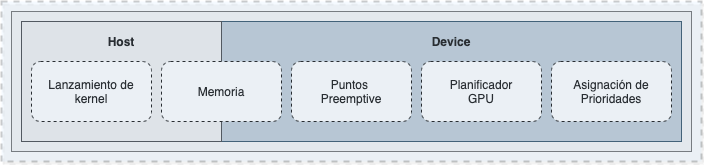
\includegraphics[scale=.6]{diagrama_framework}
        \caption{Esquema del framework para la planificación de tareas preemptive en sistemas embebidos heterogéneos.}
        \label{fig:diagramabase}
    \end{figure}
  
  %Pero en el momento en el que se requiera tener un método de asignación de prioridades personalizado, es necesario tener un módulo que lo permita. Aunado a esto, si por alguna razón se solicita agregar tareas dinámicamente con el sistema en ejecución, se deben tener mecanismos para manejar cualquier interrupción o actualización de información del planificador. Ambos elementos son necesarios en un framework, pero sus componentes internos se dejarán para ser resueltos como trabajo futuro.
  
  %Clasificación y tipo de modificación.

Como se detallará más adelante, esta solución no es transparente al programador, es necesaria la modificación del código fuente. Aunque en un inicio pareciera que el rendimiento es inferior al realizar comprobaciones continuas del estado del quantum, la modificación de las bibliotecas del API o el compilador del dispositivo y la implementación de analizadores sintácticos para la lectura de directivas precompiladas salen de las posibilidades de acción del proyecto, 
por eso no es necesario modificar el código fuente para colocarlas.
\newline 

El diseño del planificador está fuera del contexto de esta tesis, pero se puede implementar con cualquiera en la gama de algoritmos del estado del arte (ver sección \ref{sec:AlgoPlan}).

  \begin{figure}[!]
      \centering
     % \flushleft
        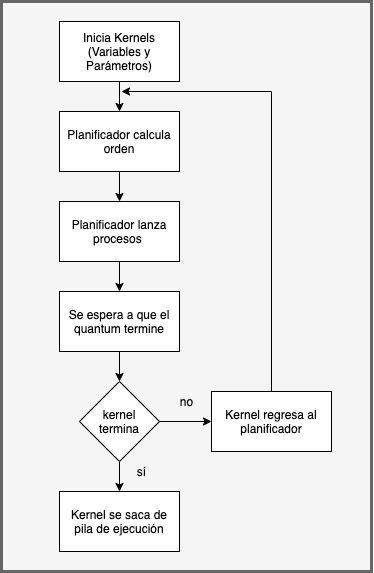
\includegraphics[scale=.58]{flujo}
        \caption{Diagrama del flujo del framework.}
        \label{fig:flujo}
    \end{figure}

\subsection{Precondiciones necesarias} \label{secc:precondiciones}

\begin{itemize}
\item La precondición más importante radica en que el framework debe ser implementado en un programa que funciona correctamente, ya que se realizará una modificación en su código fuente para la implementación del modo preemptive.

\item No se permite la memoria dinámica ni compartida entre kernels.

\item No se permiten apuntadores complejos. 

\item No se permite el llamado a funciones no rastreables.

\item El quantum de las tareas debe ser similar para que aquellas que estén en ejecución terminen en tiempos similares.

\item El número de threads por block debe ser menor o igual a la cantidad de threads disponibles en cada SM.

 \item Los contextos de cada kernel deben poder coexistir en la memoria al mismo tiempo para que se puedan ejecutar y suspender en cada punto preempetive.

\item Todas las tareas que soliciten recursos al planificador deben ser preemptive para que en dado caso puedan ser suspendidas, si así lo requiere el balanceo de carga.

\item Para evitar en la medida de lo posible plazos vencidos, el conjunto de tareas debe ser planificable.

\end{itemize}

\section{Puntos preemptive}\label{secc:puntosPreemptive}

%Descripción general del módulo.

En una aplicación acelerada por el cómputo gráfico muchas veces se implementan más de una función kernel, y en el momento en que ejecutamos varias aplicaciones en la GPU habrá alguna que mantenga en sobretiempo los recursos causando así un retraso en la ejecución en general de todo el sistema.
\newline

Este módulo permite gestionar la actividad de un kernel a nivel de aplicación, aquí se marca la pauta el punto exacto donde se podrá realizar la administración del contexto de una tarea en ejecución, contará con tres casos principales: si se está iniciando el proceso, si está a la mitad de una ejecución o si ya ha terminado, con esto se podrán liberar las unidades de procesamiento para dar lugar a otras tareas de consumir recursos.
\newline

Se propone una serie de puntos de control que se incluirán explícitamente dentro del código que se desea implementar en modo preemptive, esto durante básicamente tres etapas iterativas del ciclo de vida de un kernel a)inicio, b)en ejecución y c)finalización. 
\newline

El objetivo de este bloque es guardar una copia del contexto actual en una estructura de datos cada que se alcance algún punto de control dentro de un kernel y sea necesario detener su ejecución. De esta manera, cuando se  presente una nueva oportunidad de ejecución sea reanudado como si no se hubiera detenido.
\newline

Una vez que una tarea, independientemente del momento de su ciclo de vida en que se encuentre, seguirá ejecutándose en la GPU hasta que complete su cálculo o termine su quantum.
\newline

Al momento de lanzar la tarea siguiente en ejecución se inicializaran todas las variables necesarias en el nuevo contexto por medio de estructura copia de seguridad. Cuando se está en la etapa de inicio de un kernel se inicializan los datos necesarios para el funcionamiento de éste, tanto en su cuerpo, como  en la estructura de datos.
\newline
%Qué especificación tiene y cómo se maneja?

Al inicio del algoritmo \ref{lst:declara} la función kernel está ligeramente modificada en sus parámetros, ya que es necesario que reciba la estructura \textit{Backup} en donde se almacenará su contexto cuando se presente una suspensión preemptive y se recibirá el apuntador al estado del quantum, dicho valor arrojará \textbf{\textit{true}} cuando se haya concluido el tiempo del quantum.
\newline

Como se mencionó anteriormente, esta solución se basa completamente en software, por lo que se debe modificar la función kernel para mantener una convención que ayude a mitigar posibles problemas. Todas las declaraciones de variables deberán realizarse en la primera fase, la cual se encuentra en las primeras líneas del kernel.
\newline

Las únicas declaraciones con inicialización permitidas en esta fase son aquellas que designan la posición tanto de los thread como de los blocks dentro de un grid, esto porque  su información es necesaria en cada una de las siguientes fases. La única variable que es necesaria para todos kernels es \textit{id\_block}, que servirá en las siguientes fases para extraer la información de la estructura \textit{Backup}.

\lstinputlisting[style=CStyle, frame=single,label=lst:declara,  basicstyle=\ttfamily\footnotesize, caption=Fase de declaración de variables.]{algorithms/fase_declaracion.c}

Enseguida pasamos a la fase de la inicialización (ver algoritmo \ref{lst:declara}) de cada una de estas variables y como se muestra en el algoritmo \ref{lst:inicializa} nos apoyamos de una estructura \textit{switch-case} con tres casos dependiendo del estado de cada block. Para seleccionar cada uno de los casos debemos leer el valor que se encuentra en la estructura de copia de seguridad, esto porque hay que recordar que el kernel por si solo no sabe si es la primera vez que se ejecuta o es el producto de un cambio de contexto dentro del sistema.
\newline

Los tres estados son:

\begin{itemize}
\item \textit{\textbf{INICIO}}: Es el primer estado, y se presenta la primera vez que es lanzado un kernel, por lo que el valor inicial debe ser almacenado tanto en la variable local como en su espacio correspondiente en la estructura de copia de seguridad.

\item \textit{\textbf{EJECUCION}}: Este estado se presenta una vez inicializadas las variables en el caso anterior, o cuando el planificador da nuevamente oportunidad de ejecución para terminar el procesamiento. Aquí se realiza una transacción de memoria con los datos de la estructura de copia de información a las variables locales para trabajar con la información como si nunca se hubiera suspendido el kernel.

\item \textit{\textbf{TERMINADO}}: Debido a que muchas veces dentro de un kerel hay blocks que finalizan su procesamiento antes que otros, es necesario indicar que esa sección ya terminó y no requiere hacer ningún cálculo.
\end{itemize}

\lstinputlisting[style=CStyle, frame=single,label=lst:inicializa,  basicstyle=\ttfamily\footnotesize, caption=Fase de inicialización.]{algorithms/fase_inicializa.c}

Una vez inicializadas todas las variables podemos realizar el procesamiento objetivo del kernel (ver algoritmo \ref{lst:inicializa}). Para ello, nuevamente preguntamos a la estructura de copia de seguridad el estado individual de cada block, dependiendo de lo que responda a cada uno, se realiza lo siguiente:

\lstinputlisting[style=CStyle, frame=single,label=lst:procesamiento,  basicstyle=\ttfamily\footnotesize, caption=Fase de procesamiento.]{algorithms/fase_procesamiento.c}

\begin{itemize}
\item \textit{\textbf{INICIO}}: Como se acaba de lanzar el kernel por primera vez, únicamente se cambia el estado del block a \textit{EJECUCION}, y, como ahora se tiene un nuevo valor se puede ingresar al siguiente estado dentro del mismo switch.

\item \textit{\textbf{EJECUCION}}: Al entrar en este caso, en primera instancia se realiza el paso de procesamiento para resolver una parte del kernel original, esto dentro de una estructura \textit{do-while} para que al menos se realice una vez antes de que, o el quantum haya expirado, o se haya completado el procesamiento. Si una de estas condiciones se cumple, el ciclo se rompe, y se pregunta si ya se completo el procesamiento. Si es así, el estado del block en el backup se modifica a \textit{TERMINADO} y finaliza ese block sin realizar copia de seguridad para ahorrar tiempo de procesamiento.
En caso de que no haya sido completado, significa que el quantum expiró, por lo que se deben guardar todas las variables locales en su espacio correspondiente designado dentro del backup. Terminado esto, se finaliza el block.

\item \textit{\textbf{TERMINADO}}: En el supuesto que se llegue a este caso, significa que se lanzó nuevamente el kernel porque existen blocks que aún no terminan su trabajo, por lo que éste simplemente termina su ejecución.
\end{itemize}



\subsection{Condición de carrera}

La fase de procesamiento (ver algoritmo \ref{lst:procesamiento}) es un procedimiento en el que hay que poner especial atención, ya que es donde se concentra el núcleo de las operaciones del kernel, además es donde se escriben variables compartidas por todo el grid. Por ello, hay que estar conscientes de que se debe evitar la condición de carrera.
\newline

Por esta razón, en el \textit{case INICIO} únicamente el \textit{thread0} de cada block está habilitado para modificar el estado que se guarda en el \textit{backup}. Justo después del cambio de estado se debe esperar en una barrera para que todos los thread conozcan la actualización y no terminen abruptamente su procesamiento.
\newline

Lo anterior se repite en el \textit{case EJECUCION}, cuando se termina el procesamiento, nuevamente sólo el \textit{thread0} está autorizado para editar el contenido del arreglo \textit{estado} en la estructura de copia de información.
\newline

Finalmente, si el procesamiento se realiza con ayuda de contadores, al momento de que expire el quantum, todos los threads deberán suspenderse cuando lleguen al mismo valor, así que, lo más conveniente (en términos de memoria) es guardar sólo una copia de dicho contador. Entonces, una vez más el \textit{thread0} será quien almacene la información en su correspondiente lugar dentro de \textit{thread0}.

%%%%%%%%%%%%%%%%%%

  \section{Memoria}\label{secc:memoria}

  \subsection{Almacenamiento del contexto}
%Descripción general del módulo.

Es necesario crear una estructura de datos que guarde las copias de seguridad de los datos pertinentes que en conjunto formen el contexto de un kernel.
\newline

Todos los parámetros y variables que se encuentren dentro de una función kernel deben almacenarse en memoria, por lo que para cada uno de los kernel, se debe crear una estructura \textit{ad hoc}.
\newline

\lstinputlisting[style=CStyle, frame=single,label=lst:backup,  basicstyle=\ttfamily\footnotesize, caption=Estructura Backup para almacenar el contexto.]{algorithms/backup.c}

La estructura \textit{backup} (ver algoritmo \ref{lst:backup}) almacena tres tipos de valores, primero todas aquellas variables locales necesarias para resolver el problema original del kernel. Debido a que estas variables son individuales por thread, debe guardarse una copia de cada thread por cada bloque. Esta solución es muy costosa, por lo que se recomienda que la utilización de estas variables sea mínima o nula. En muchos casos, podría almacenarse su contenido directamente en alguna de las variables \textit{resultado} que se pasaron como parámetro.
\newline

El segundo tipo de variables es el de tipo contador. Dependiendo del cálculo que se esté realizando, muchas veces se deberán paralelizar \textit{estructuras for} sin dependencia de datos.  Por esta razón, puede que después de un cierto número de iteraciones se pregunte por el estado del quantum, y ,en ese momento, se realice la suspensión preemptive para todos los threads de un block. Como todos llegaron a ese punto, simplemente, se puede  guardar un valor del contador. En caso de que se estén utilizando contadores que son propiamente controlados por un punto de verificación de quantum, se deberá utilizar el formato de variable local.
\newline

Finalmente, debemos incluir un arreglo más que nos ayude a guardar el estado en que se quedó un block al ser detenido por el planificador.

  \subsection{Variables compartidas}
  
  Al momento de realizar una solución de GPGPU, tenemos que  considerar que existirán variables que deben mantenerse visibles tanto para el host como para el device. En el algoritmo \ref{lst:lanzamiento} de la sección \ref{secc:lanzamientoKernel} tenemos ciertas variables que deben ser compartidas entre ambos lados. 
    \newline
  
  Aparte de los parámetros que originalmente tienen la función kernel, se agregan dos más: una estructura \textit{backup}, que almacena el contexto cuando se presenta una suspensión preemptive, y ,la bandera \textit{quantum\_expirado}, que nos indica si ya terminó el tiempo máximo de ejecución. Como estamos en el dominio de la memoria unificada, ambos parámetros existirán en la memoria global para que estén disponibles para ambos dispositivos.
  
  
  %%%%%%%%%%%%%%%%%%%%%%%%%%%%%%%%%%%%%%%%%%%%%%%%%%%%%%%%%%%%%

\section{Lanzamiento del kernel}\label{secc:lanzamientoKernel}

El framework plantea dos precondiciones estrechamente relacionadas (ver \ref{secc:precondiciones}). La primera, es que el framework planificará un número estático de kernels conocidos desde el inicio y, la segunda, es que el código fuente esté disponible para su adecuación al sistema.
\newline

Cada una de las aplicaciones GPGPU que se ejecutarán en el sistema embebido deberán estar agrupadas en cabeceras de C. Al inicio de la ejecución del framework, se ejecutarán las aplicaciones de forma concurrente (Figura \ref{fig:appN_h}) para que todas alcancen el punto en que requieren realizar cálculos en la GPU.

  \begin{figure}[!]
      \centering
     % \flushleft
        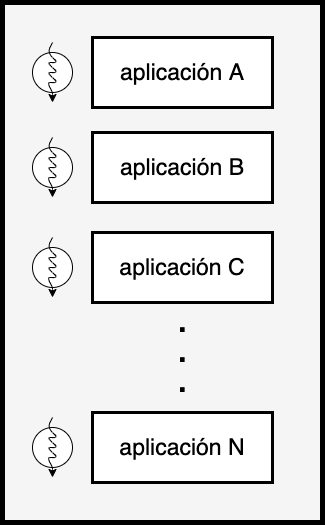
\includegraphics[scale=.3]{appN_h}
        \caption{Aplicaciones en ejecución concurrente en el CPU.}
        \label{fig:appN_h}
    \end{figure}

Al código de cada una de las aplicaciones se le debe añadir una serie de variables y parámetros para que el planificador pueda programar su ejecución. 
\newline

Se debe encapsular la llamada a la función kernel para que el planificador permita dar el orden de lanzamientos. Dentro de cada enclave se debe implementar una serie de variables y banderas para que el contexto pueda ser almacenado al alcanzar a cada punto preemptive. 
\newline

Es necesaria la definición de la estructura \textit{backup} específica del kernel, también se debe indicar la duración del quantum con \textit{quantum\_time}, una bandera de control para verificar si ya ha expirado el quantum y una bandera que indicará si ya se ha ejecutado completamente el kernel. Finalmente, el planificador dará permiso de que se ejecute el kernel con la variable de control \textit{continuar\_eje}.
\newline

Ahora bien, una vez que se han definido las variables de control, se debe implementar un ciclo que terminará hasta que el kernel sea completado. Dentro debemos inicializar \textit{quantum\_expirado} en \textbf{\textit{false}} para indicar que se tiene tiempo de ejecución. La bandera \textit{continuar\_eje} será modificada por el planificador para permitir la ejecución del kernel. Una vez que sea planificado para su ejecución, se lanzará el kernel  y se esperará el tiempo definido para el quantum. Terminado este tiempo, se cambiará el estado de \textit{quantum\_expirado} a \textit{\textbf{true}} y se sincronizarán todos los threads del kernel con \textit{cudaDeviceSynchronize()} para cerciorarnos de que se terminó la ejecución del grid.

Ahora debemos cambiar el estado de \textit{continuar\_eje} a \textbf{\textit{false}} para que la tarea permanezca suspendida hasta que el planificador permita una nueva ejecución. Finalmente, se pregunta si todos los blocks completaron su trabajo.

\lstinputlisting[style=CStyle, frame=single,label=lst:lanzamiento,  basicstyle=\ttfamily\footnotesize, caption=Algoritmo para lanzamiento del kernel en el lado del host.]{algorithms/lanza_kernel.c}

Para poder determinar si un kernel ha terminado completamente su procesamiento, nos auxiliamos de la función \textit{kc} (Algoritmo \ref{lst:funcionkc}). Simplemente se pasa como parámetro el arreglo \textit{estado} de la estructura \textit{backup} y se pregunta si el estado de todos los blocks es \textit{\textbf{TERMINADO}}, regresando \textbf{\textit{true}}.

\lstinputlisting[style=CStyle, frame=single,label=lst:funcionkc,  basicstyle=\ttfamily\footnotesize, caption=Función kernel completo.]{algorithms/funcion_kc.c}

\section{Planificador} \label{secc:planificador}

El módulo principal del framework es el del \textbf{Planificador} (ver figura \ref{fig:Planificador}) porque es aquí donde se realiza toda la calendarización de las tareas a ser ejecutadas en la GPU. Trabaja muy estrechamente con el módulo de la asignación de prioridades, el cual le da la pauta para poder elegir aquella tarea que tenga mayor relevancia en un momento determinado en el tiempo. 

\lstinputlisting[style=CStyle, frame=single,label=lst:Task,  basicstyle=\ttfamily\footnotesize, caption=Estructura task.]{algorithms/Task.c}

Para poder planificar un conjunto de tareas en la GPU, es necesario conocer las particularidades de la arquitectura del sistema embebido en el que se implementará el framework. Esto es especialmente necesario para que conozcamos el número máximo de threads que pueden estar en ejecución concurrentemente.

    \begin{figure}[!]
      \centering
        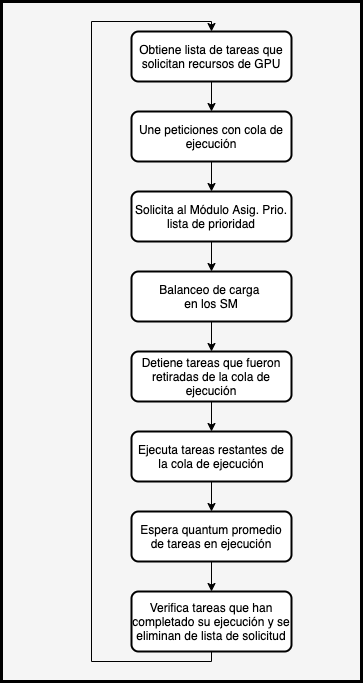
\includegraphics[scale=.6]{Planificador}
        \caption{Diagrama de flujo del planificador.}
        \label{fig:Planificador}
    \end{figure}

Cada uno de los kernels que soliciten recurso de cómputo en la tarjeta gráfica al planificador deberá ser mapeado a una estructura (algoritmo \ref{lst:Task}), la cual tendrá almacenados algunos de sus parámetros para ejecución, así como información relevante para la asignación de su prioridad en un instante de tiempo.
\newline

El algoritmo \ref{lst:planificador} muestra la manera en que deberá guiarse el programador para implementar el planificador, primero se obtiene la lista de tareas \textit{sol} que solicitan los recursos del GPU y las une con aquellas que ya se tenían en la cola de ejecución \textit{R}, esta cola contiene tanto las tareas que en una ejecución fueron beneficiadas de consumir recursos como aquellas que se mantienen en estado de ociosidad.

Se llama al módulo Asignación de Prioridad (ver sección \ref{secc:asigPrioridad}) para que devuelva la cola ordenada por prioridad \textit{r} (el orden depende del algoritmo de asignación de prioridades en tiempo real seleccionado).

La cola \textit{r} se envía a un balanceador de carga que ayudará a la maximización de la planificación de tareas ejecutables en un quantum. Posteriormente, detendrá la ejecución de aquellas que deban drenar su contexto en la iteración actual \textit{j} para darle lugar a una con mayor prioridad.
Se esperará un quantum \textit{x} (el estudio del quantum más apropiado queda fuera del contexto de esta tesis) y una vez alcanzado el plazo límite, se eliminarán de \textit{R} aquellas tareas que completaron su ejecución en la iteración \textit{j}. 

\lstinputlisting[style=CStyle, frame=single,label=lst:planificador,  basicstyle=\ttfamily\footnotesize, caption=Función planificador.]{algorithms/planificador.c}

\subsection{Balanceador de carga} \label{secc:balanceador}

Bajo suposición y asignación de una carga de trabajo, todas las tareas son preemptive debido a que por decisiones del hardware muchas veces no podrán asignarse aunque haya espacio para su ejecución.
\newline

Como se mencionó en el capítulo \ref{cha:TrabajoRelacionado} el orden de lanzamiento de los kernel a la GPU afecta la forma en que serán asignados a los SM. Por ejemplo, en el escenario a) (ver figura \ref{fig:Balanceo}). Primero se lanza \textbf{K1}, seguido de \textbf{K2} y al final \textbf{K3}, dando como resultado el desperdicio de recursos y que no sea posible ejecutar un kernel. Sin embargo, si se modifica este orden, se puede optimizar la asignación de tareas en las localidades, como lo vemos en el ejemplo b).
\newline

Por esta razón, se ideó un balanceador de carga (ver algoritmo \ref{lst:Balanceador}) que permitirá la maximización de la planificación de tareas ejecutables en un quantum.
\newline

        \begin{figure}[!h]
      \centering
        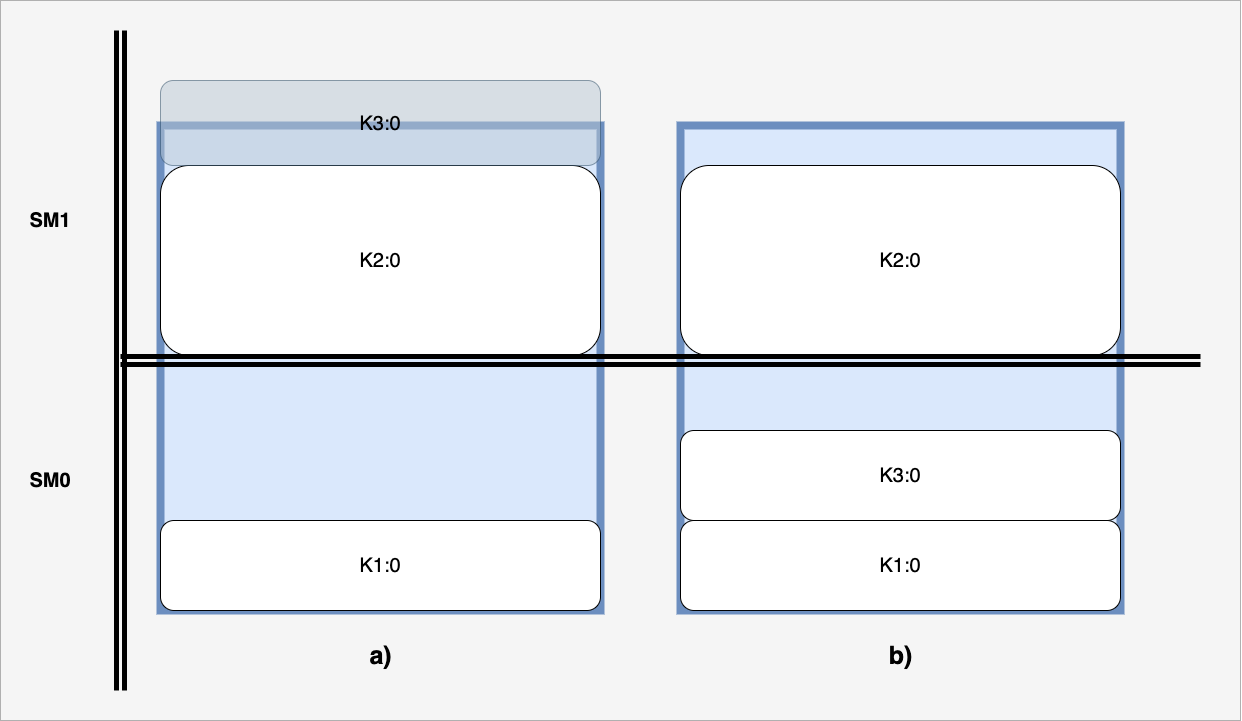
\includegraphics[scale=.24]{Balanceo}
        \caption{Diagrama de balanceo de carga de kernels en los SM.}
        \label{fig:Balanceo}
    \end{figure}
    
    Como se ha visto a lo largo de este trabajo, la asignación de recursos para la ejecución de kernels en la tarjeta gráfica no es algo trivial, por lo que fue necesario diseñar un balanceador de carga (ver figuras \ref{fig:Balanceador1} y \ref{fig:Balanceador2}) que tomará en cuenta las características propias del sistema utilizado como caso de estudio.
    \newline
    
    Debido a que las tareas que serán ejecutadas sobre el sistema se presuponen embebidas, se considera que probablemente podrán ejecutarse al menos dos kernels en concurrente sobre la tarjeta, por lo que es imprescindible que ellas siempre tengan recursos suficientes para su ejecución. En caso de que la tarea de mayor prioridad absorba todos los recursos, no será necesario ejecutar la segunda tarea en ese quantum.
\newline

    \begin{figure}[!]
      \centering
        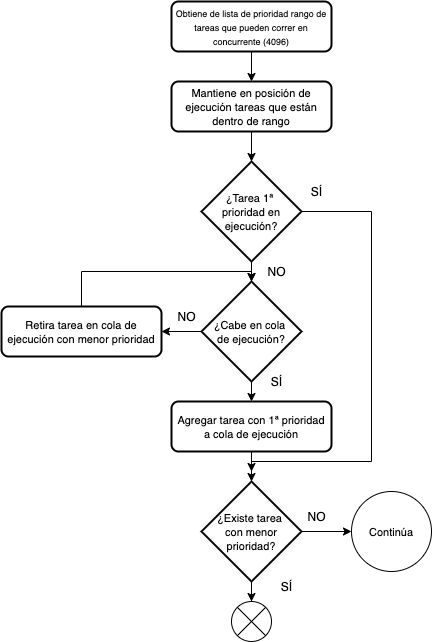
\includegraphics[scale=.7]{Balanceador1}
        \caption{Diagrama de flujo del balanceador de carga parte 1.}
        \label{fig:Balanceador1}
    \end{figure}
    
    \begin{figure}[!]
      \centering
        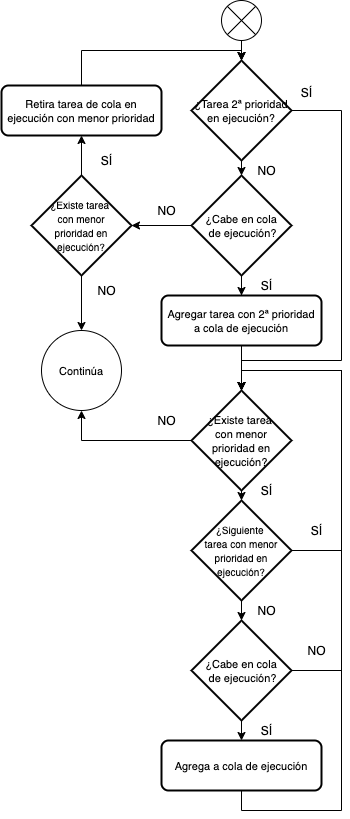
\includegraphics[scale=.7]{Balanceador2}
        \caption{Diagrama de flujo del balanceador de carga parte 2.}
        \label{fig:Balanceador2}
    \end{figure}

    \lstinputlisting[style=CStyle, frame=single,label=lst:Balanceador,  basicstyle=\ttfamily\footnotesize, caption=Balanceador de carga.]{algorithms/balanceoCargav3.c}

La lógica de asignación de tareas a los SM se basa en colocar la mayor cantidad posible de kernels en concurrente para que se puedan realizar más cálculos en menor tiempo.
\newline

    \begin{figure}[!]
      \centering
        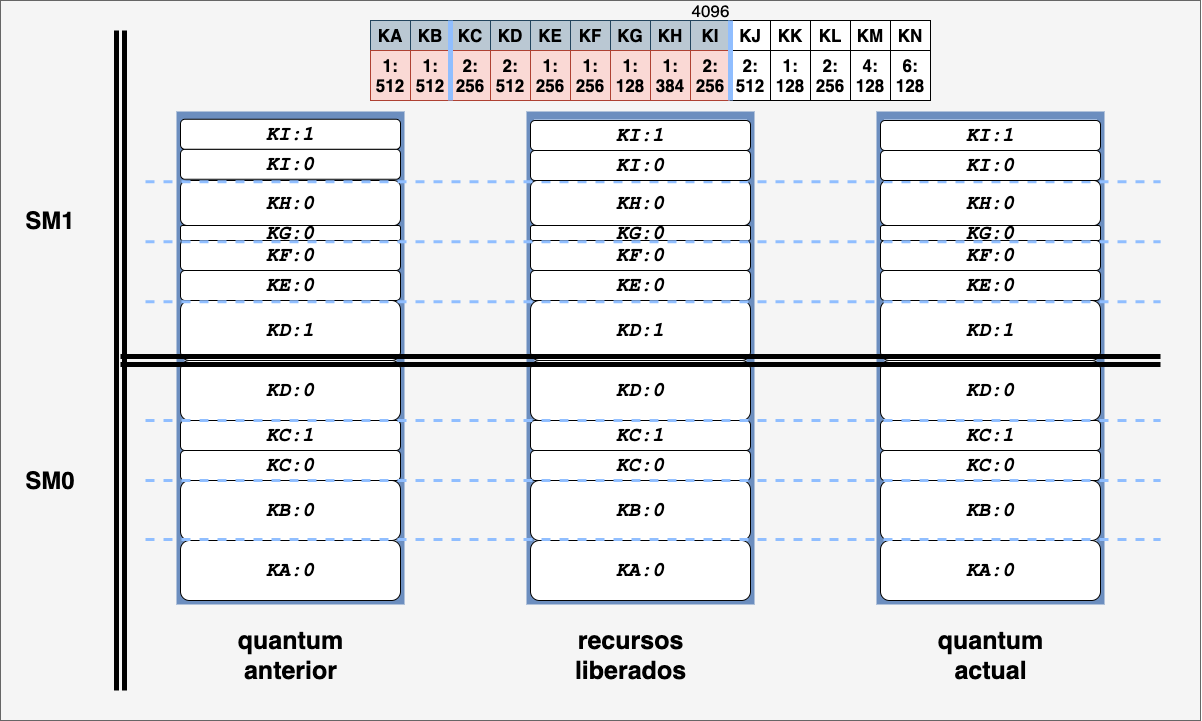
\includegraphics[scale=.26]{C1Balanceo}
        \caption{Caso I Kernels mantienen su prioridad en la siguiente iteración.}
        \label{fig:C1Balanceo}
    \end{figure}

A continuación se muestran algunos de los diversos escenarios en forma de casos de estudio que pueden aparecer al recurrir al balanceador de carga. Cada uno está representado en un diagrama, el cual posee en la parte superior la lista ordenada por prioridad (mayor a menor), cada tarea contiene el nombre del kernel así como el número de blocks que se requieren lanzar seguido del número de threads que los comprende. Se sombrean aquellas tareas que lograron ejecutarse en cada iteración, también se tiene una división en la lista. A la izquierda se comprenden las tareas que pudieran correr en concurrente en un punto en el tiempo de ejecución. A la derecha, aquellas que salen de dicha cuenta, justo en la última tarea de la primera mitad se tiene las suma de los threads que hipotéticamente pudieran ejecutarse en concurrente.
\newline

El Caso I (ver figura \ref{fig:C1Balanceo}), representa un escenario en donde la totalidad de las tareas que estaban ejecutándose en la iteración anterior a) vuelven a quedar en la posición de mayor prioridad en la lista en b), puesto que ninguna tarea tuvo que ser sacada de ejecución, se les dará oportunidad de un siguiente quantum sin necesidad de detenerse guardar su contexto y relanzarse.
    \newline
    
    \begin{figure}[!]
      \centering
        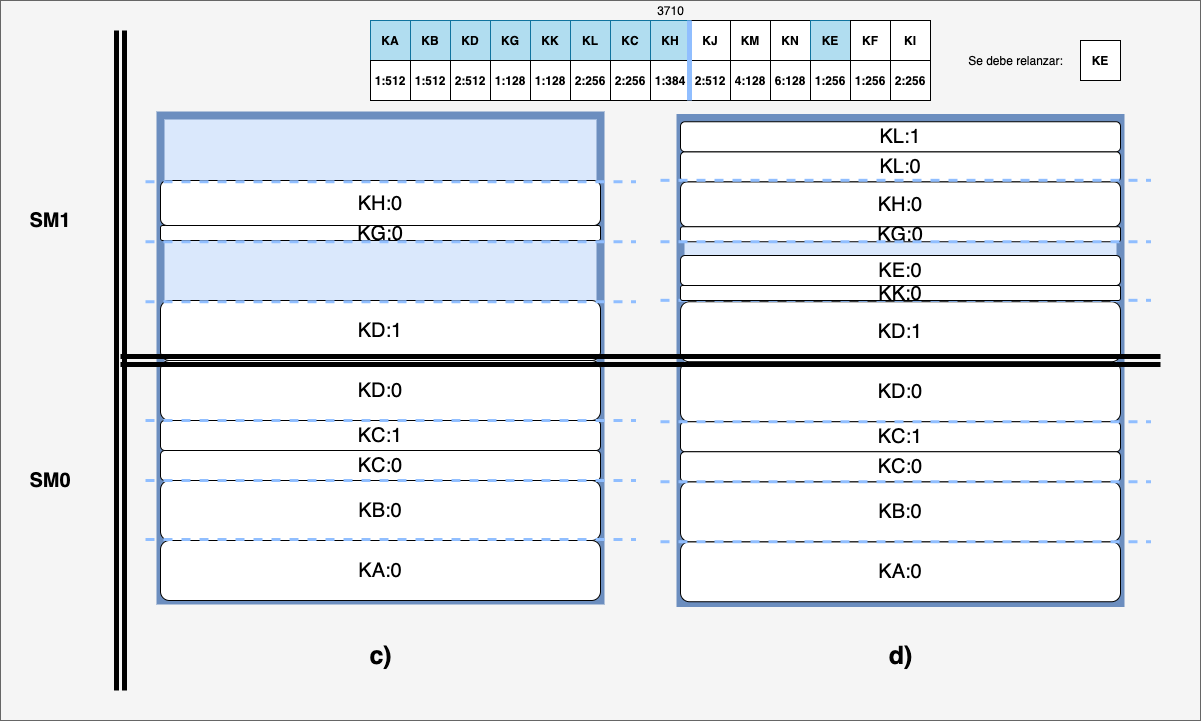
\includegraphics[scale=.26]{C2Balanceo}
        \caption{Caso II Kernels de baja prioridad deben relanzarse.}
        \label{fig:C2Balanceo}
    \end{figure}
    
    Una vez terminado el quantum de la iteración y recalculando la lista de prioridades observamos que se presenta el Caso II (ver figura \ref{fig:C2Balanceo}), donde algunas de las tareas ahora cambiaron el orden en la lista. Procedemos a calcular el rango de las tareas que pudieran correr en concurrente, y encontramos que la mayoría puede continuar en ejecución por que se encuentran del lado derecho. Aquellas que quedaron del lado derecho se deben sacar de la lista de ejecución y ser insertadas en la lista de paro de actividades para dar oportunidad de ejecución a aquellas que tienen mayor prioridad, para este caso serían los kernel \textbf{KE}, \textbf{KF} y \textbf{KI}. Luego, procedemos a agregar las del lado derecho por orden de prioridad, \textbf{Kk} y \textbf{KL}. 
    Una vez agregadas las tareas de mayor prioridad, se observa que aún queda espacio y se pregunta a las tareas de menor prioridad si sus características cumplen con los requisitos para que puedan ser ejecutadas en esa iteración, con ello concluimos que la tarea \textbf{KE} puede ingresar a ejecutarse.     
    \newline
    
    \begin{figure}[!]
      \centering
        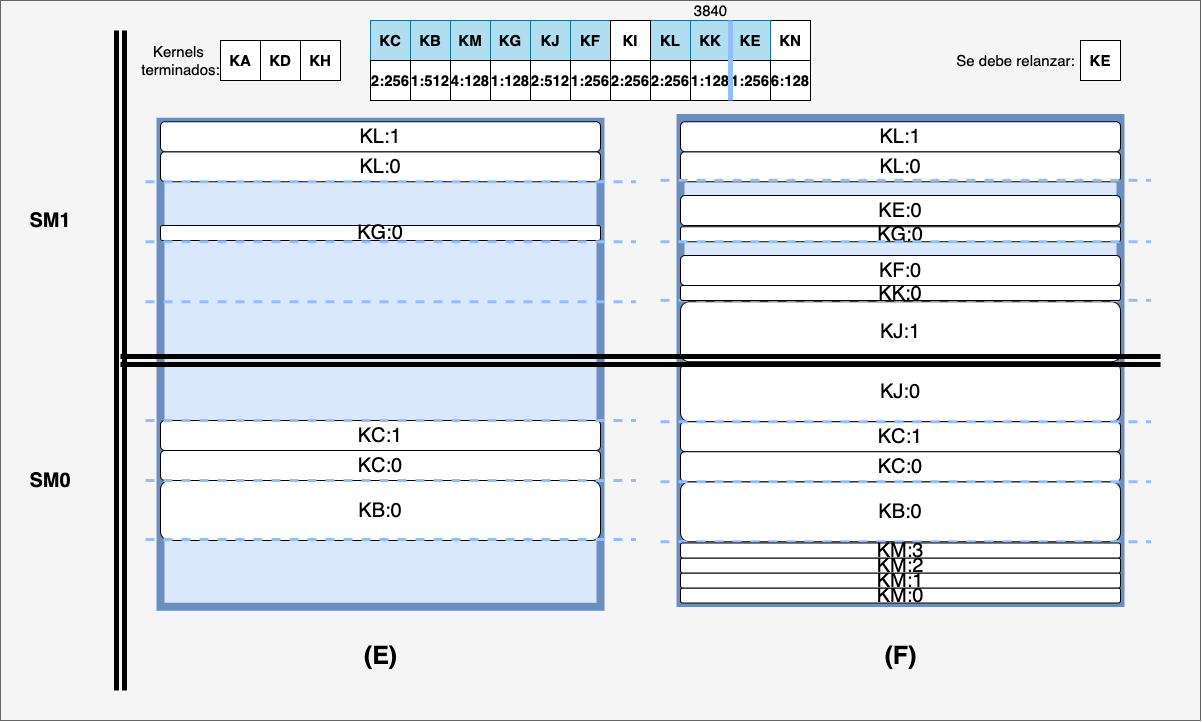
\includegraphics[scale=.26]{C3aBalanceo}
        \caption{Caso IIIa Kernels que completaron su ejecución.}
        \label{fig:C3aBalanceo}
    \end{figure}

    Después de terminada la iteración d), se encontró que las tareas \textbf{KA}, \textbf{KD} y \textbf{KH} han completado su ejecución, por lo que son eliminadas de la lista de peticiones. Por ello, la lista de prioridades para esta ejecución se modificó tanto en orden, como en longitud. Una vez calculado el rango de las posibles tareas en concurrente, encontramos que varias de ellas ya no existen, o bien, deben ser retiradas de ejecución para dar lugar a otras con mayor prioridad. En esta ocasión nos quedamos únicamente con \textbf{KB}, \textbf{KC}, \textbf{KG} y \textbf{KL}, y, procedemos a rellenar el espacio existente con las tareas según su orden de prioridad. 
    \newline
    
    \begin{figure}[!]
      \centering
        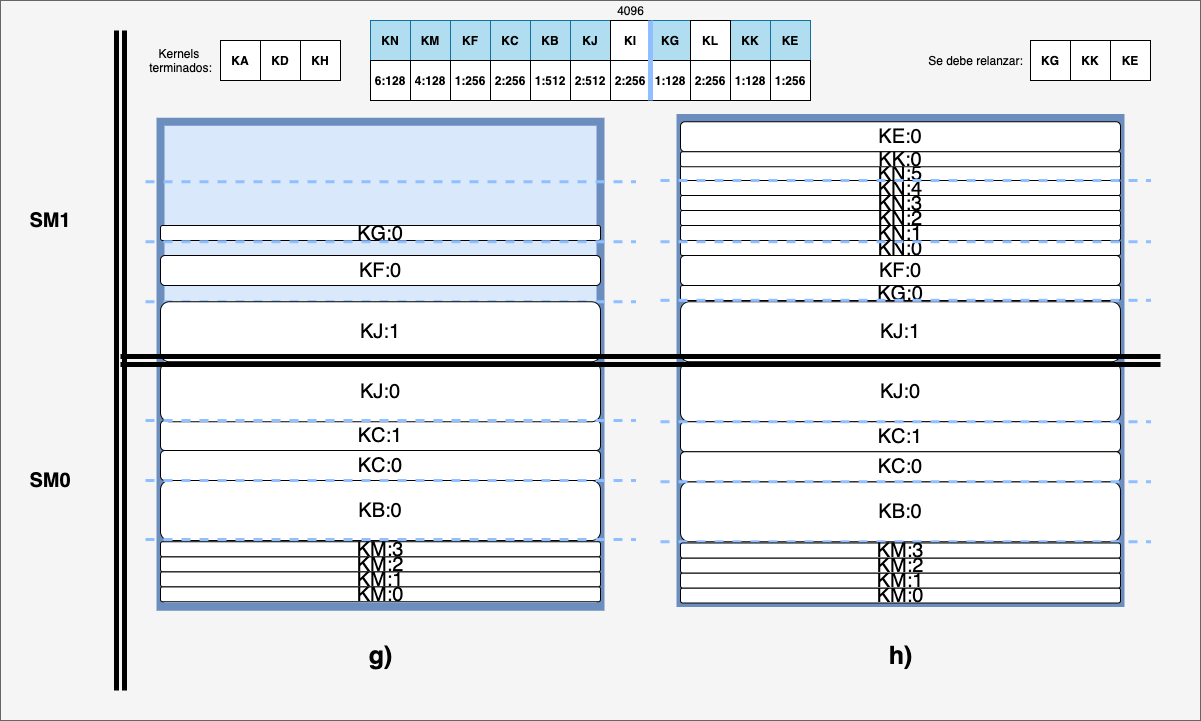
\includegraphics[scale=.26]{C3bBalanceo}
        \caption{Caso IIIb Kernels que completaron su ejecución.}
        \label{fig:C3bBalanceo}
    \end{figure}
    
    Pero en el Caso III (ver figura \ref{fig:C3aBalanceo}), debido a la forma en que están dispuestas las tareas, teóricamente la tarea \textbf{KI} debería poder ejecutarse porque hay suficientes threads para su ejecución, pero el hecho de que no estén contiguos imposibilita esta acción. 
    Por ello, se salta y se decide agregar tareas de menor prioridad, incluso \textbf{KE} que está del lado derecho de la lista de prioridad. Debido a que nuevamente tenía una baja prioridad y tuvo que ser quitada de ejecución, y, se le dió oportunidad de ejecutarse (sin importar si fuera en su misma ubicación) debe detener su ejecución, guardar su contexto y volver a ejecutarse.
\newline

    Siguiendo con el flujo del planificador, (ver figura \ref{fig:C3bBalanceo}) se vuelve a obtener una nueva lista de ejecución (nótese que del lado izquierdo se indica que se podrían utilizar los 4096 threads de los SM). Al momento de llenar la cola de ejecución por prioridad, aunque la tarea  \textbf{KI} nuevamente se queda fuera de ejecución, ahora ganamos recursos para 3 de menor prioridad \textbf{KG}, \textbf{KK} y \textbf{KE}. Como dichas tareas se encontraban en ejecución en la iteración pasada pero ahora son de baja prioridad, se deben detener para ser lanzadas nuevamente.
\newline

    \begin{figure}[!]
      \centering
        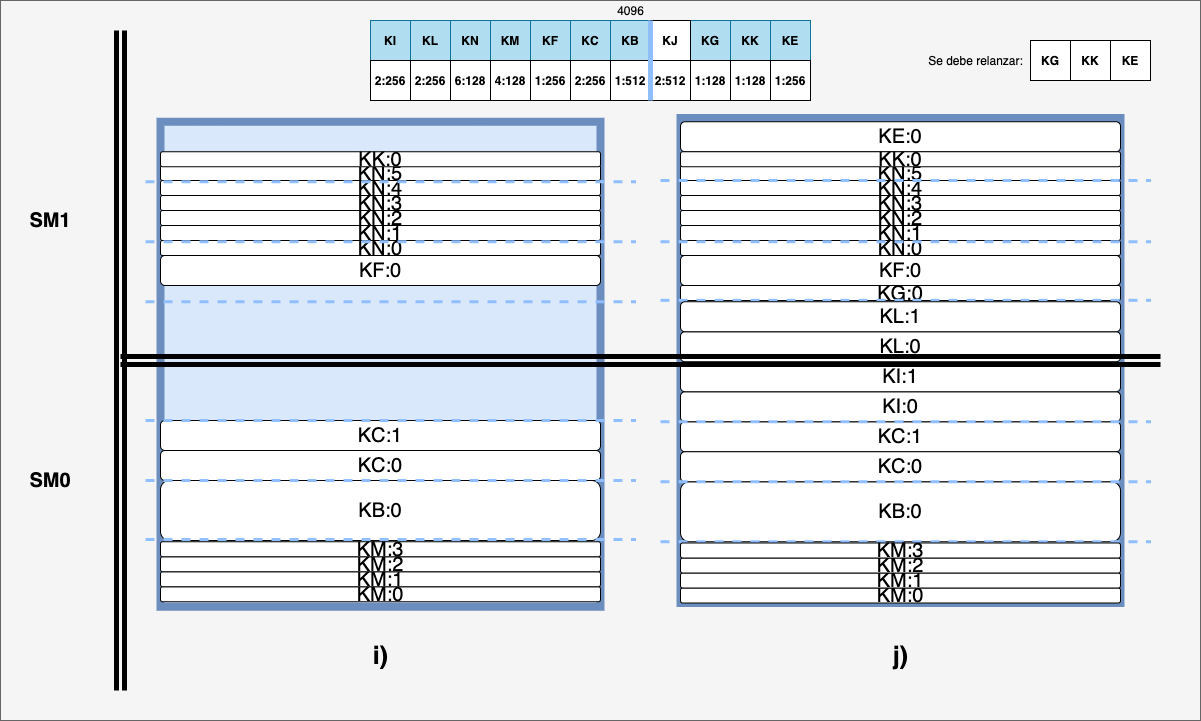
\includegraphics[scale=.26]{C4Balanceo}
        \caption{Caso IV Kernels muy grandes.}
        \label{fig:C4Balanceo}
    \end{figure}
    
    En el Caso IV (ver figura \ref{fig:C4Balanceo}) se tiene que la lista ordenada de prioridad del lado izquierdo contiene tareas que no ocupan por completo los recursos aportados por los SM, pero la primer tarea del lado derecho por sus características no puede ser ejecutada. 
    Por ello, no fue seleccionada en primer lugar, ya que es necesario empezar a llenar el espacio sobrante con las tareas de baja prioridad. En este caso, maximizamos la totalidad de los recursos de los SM y ejecutamos toda la lista de prioridad a excepción de la tarea \textbf{KJ}. Y nuevamente, como al inicio no estaban planeadas para su ejecución en esta iteración, se debe detener y relanzar a las tareas \textbf{KG}, \textbf{KK} y \textbf{KE}.
\newline

    \begin{figure}[!]
      \centering
        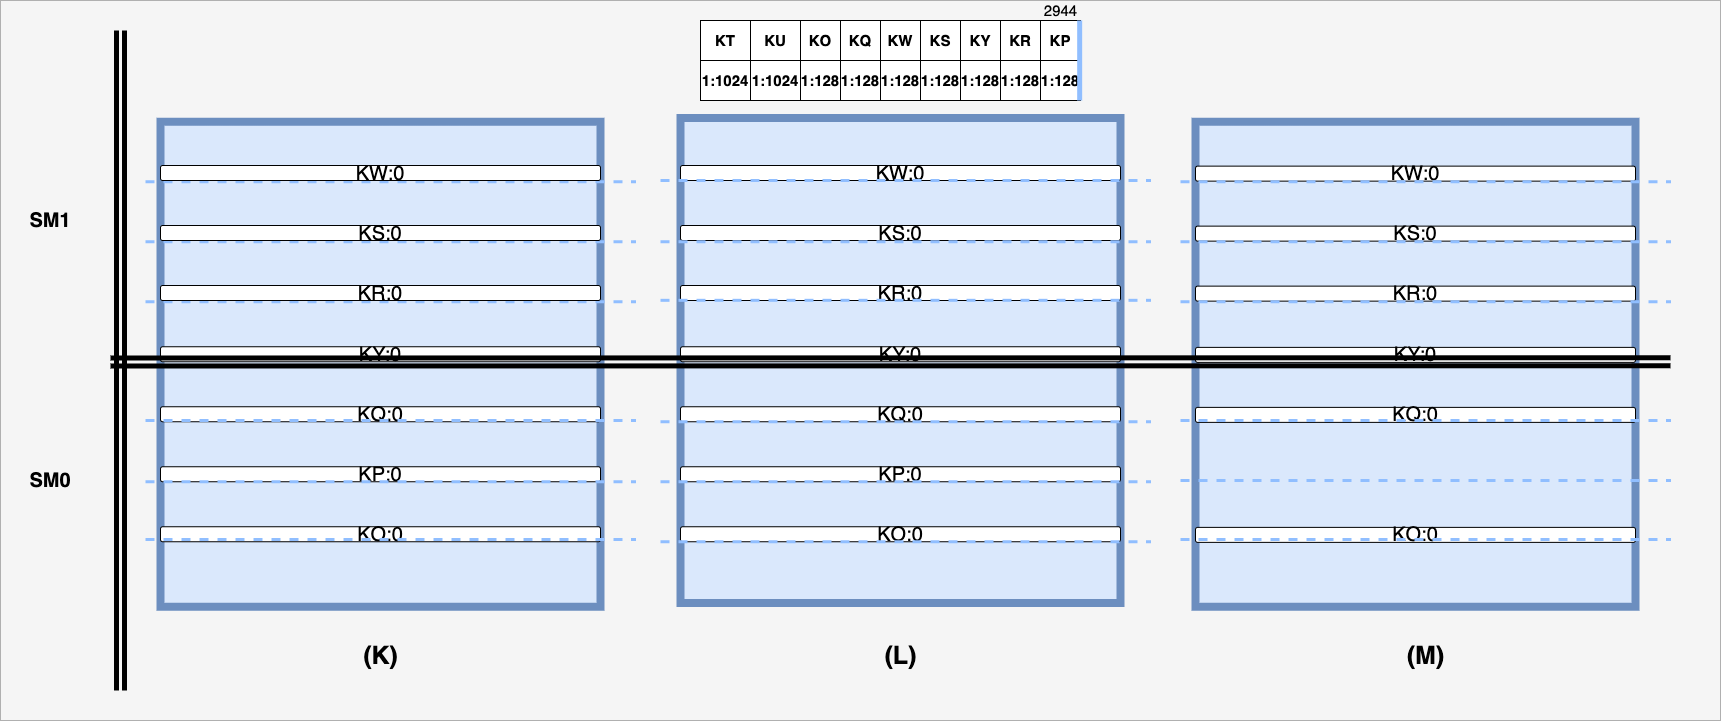
\includegraphics[scale=.25]{C5aBalanceo}
        \caption{Caso Va Kernels de mayor prioridad que no estaban en ejecución.}
        \label{fig:C5aBalanceo}
    \end{figure}
    
    \begin{figure}[!]
      \centering
        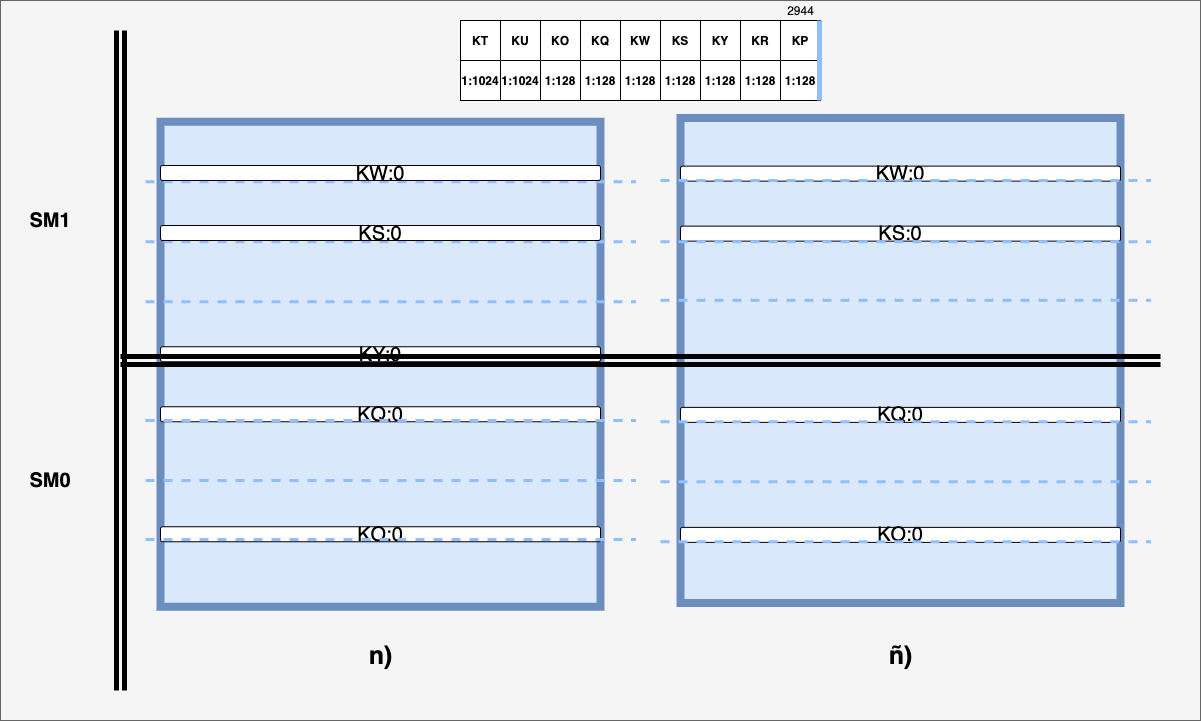
\includegraphics[scale=.26]{C5bBalanceo}
        \caption{Caso Vb Kernels de mayor prioridad que no estaban en ejecución.}
        \label{fig:C5bBalanceo}
    \end{figure}
    
    Después de diversas iteraciones del ciclo de vida del planificador, nos encontramos con el escenario k) (ver figura \ref{fig:C5aBalanceo}), donde tenemos que se encuentran en ejecución un cierto número de tareas esparcidas por los SM que utilizan solamente una fracción de sus recursos. Justo después de que se acaba el quantum de su iteración, se calcula nuevamente la lista de prioridad en l),y, ahora han aparecido dos tareas en la cabeza de la cola que solicitan recursos.
    Debido a que la de mayor prioridad no puede recibir recursos contiguos para su ejecución, se procede a sacar la tarea de menor prioridad actualmente en ejecución \textbf{KP}, y la de mayor prioridad pregunta nuevamente si ahora puede entrar en ejecución.
\newline

    Como no es posible que ingrese, se vuelve a quitar de ejecución la tarea con la menor prioridad (ver figura  \ref{fig:C5bBalanceo}), y así sucesivamente hasta que se reúnan las características que se requieren. Una vez liberado el espacio en ñ), se añade la tarea con la mayor prioridad en o), y se pregunta ahora por el espacio requerido por la tarea con la segunda mayor prioridad. Como nuevamente no se puede agregar a ejecución, se eliminan las tareas de menor prioridad hasta que sea posible colocarla.
\newline

    \begin{figure}[!]
      \centering
        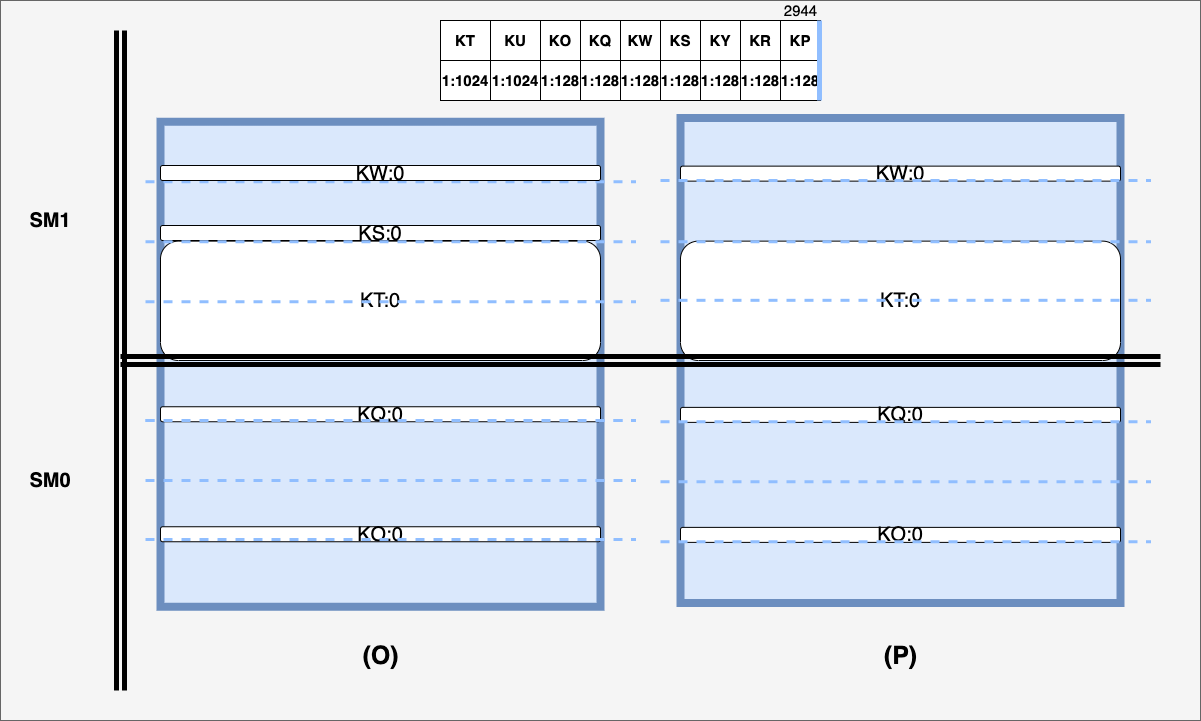
\includegraphics[scale=.26]{C5cBalanceo}
        \caption{Caso Vc Kernels de mayor prioridad que no estaban en ejecución.}
        \label{fig:C5cBalanceo}
    \end{figure}

    Una vez liberado el espacio contiguo necesario para la tarea \textbf{KT}(ver figura  \ref{fig:C5cBalanceo}), y así sucesivamente hasta que se reúnan las características que se requiere. Una vez liberado el espacio en ñ), se añade la tarea con la mayor prioridad en o), y se pregunta ahora por el espacio requerido por la tarea con la segunda mayor prioridad, como nuevamente no se puede agregar a ejecución, se eliminan las tareas de menor prioridad hasta que sea posible colocarla.
\newline
    
    \begin{figure}[!]
      \centering
        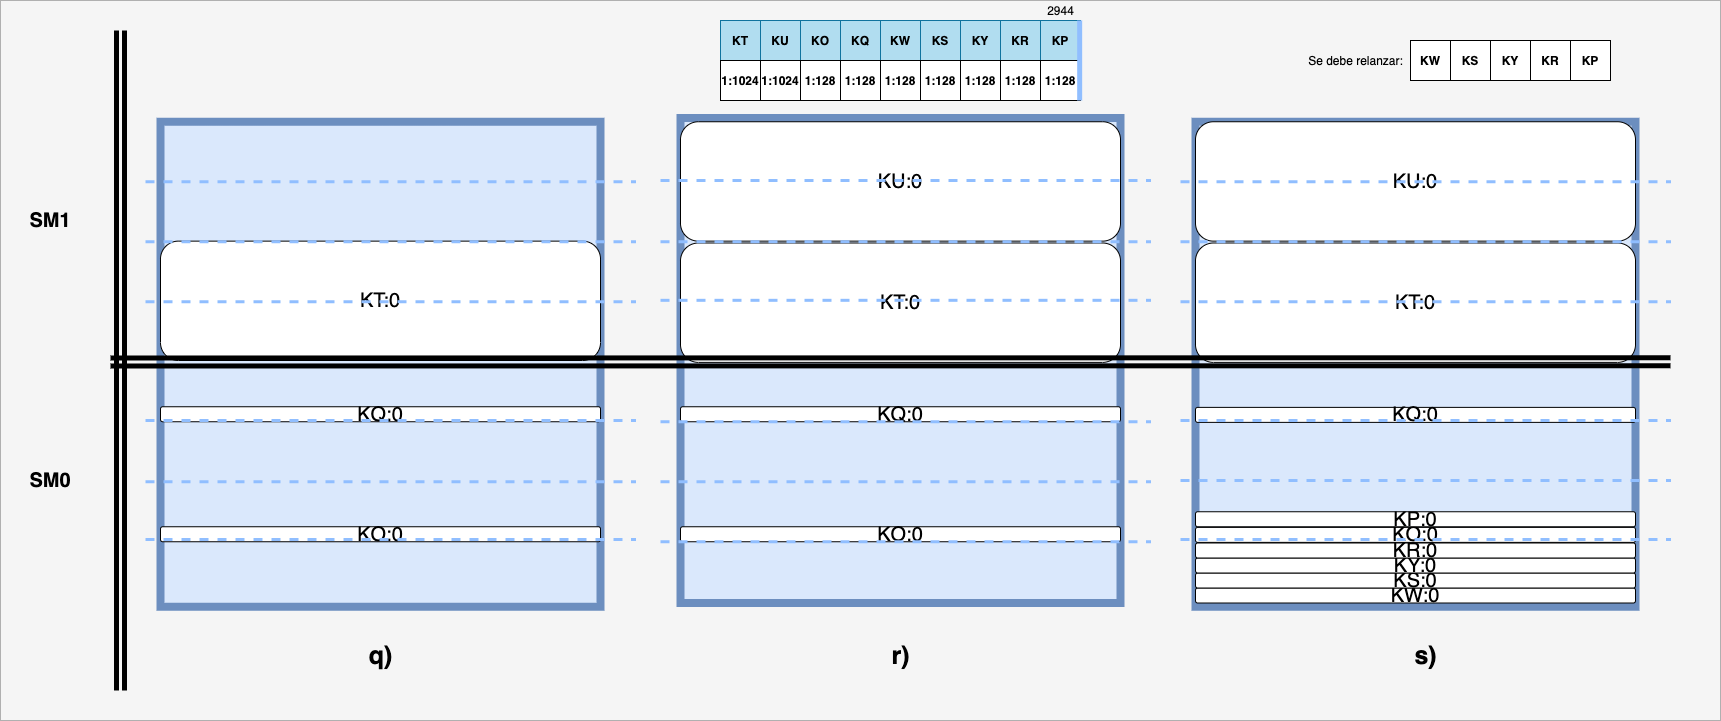
\includegraphics[scale=.26]{C5dBalanceo}
        \caption{Caso Vd Kernels de mayor prioridad que no estaban en ejecución.}
        \label{fig:C5dBalanceo}
    \end{figure}

   Liberado el espacio necesario (ver figura  \ref{fig:C5dBalanceo}), se procede a colocar la tarea \textbf{KU} y, posteriormente, se rellena el espacio con las tareas de la lista ordenada. Como se sacaron de ejecución las tareas \textbf{KW}, \textbf{KS}, \textbf{KY}, \textbf{KR} y \textbf{KP}, y después entraron nuevamente a la lista, es necesario relanzarlas.
\newline

    \begin{figure}[!]
      \centering
        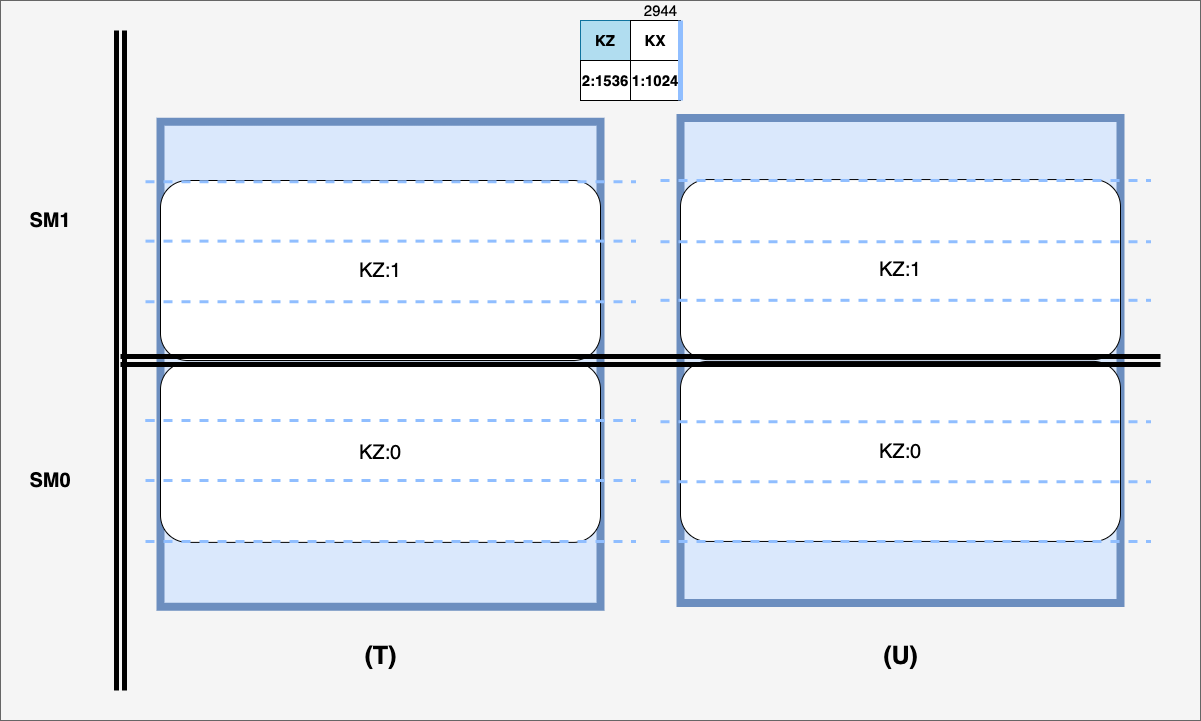
\includegraphics[scale=.26]{C6Balanceo}
        \caption{Caso VI.}
        \label{fig:C6Balanceo}
    \end{figure}
    En el Caso VI (ver figura  \ref{fig:C6Balanceo}), encontramos en q) que la tarea \textbf{KZ} ya se encontraba en ejecución, pero en la siguiente ejecución, se presentó la tarea \textbf{KW} con una prioridad menor, aunque teóricamente ambas tareas podrían ejecutarse concurrentemente, una tarea con menor prioridad no puede mover a una de mayor, por lo que en esta iteración únicamente se quedará en ejecución la tarea con la mayor prioridad.
    
\section{Asignación de prioridades} \label{secc:asigPrioridad}

Al tener como módulos separados tanto el planificador como la asignación de prioridades, nos da la flexibilidad de poder implementar diferentes algoritmos de tiempo real (ver \ref{sec:AlgoPlan}).
\newline

Para el diseño de este framework, se tomó como base el uso de algoritmos de asignación de prioridades en tiempo real de soporte monoprocesador, aunque no se descarta la posible implementación de aquellos que trabajan con multiprocesadores y subconjuntos de tareas. En este caso se asegura la ejecución de al menos dos tareas en concurrente en la tarjeta gráfica.
\newline

Dependiendo de las particularidades de cada algoritmo, se requerirá diferente información sobre la tarea a planificar, dichos parámetros podrán modificarse en la estructura (algoritmo \ref{lst:Task}) que mapea a las tareas.
\newline

Este módulo generará una lista de prioridad ordenando las tareas de mayor a menor, según sea el caso.
\newline

A cada iteración del planificador se asigna una prioridad a las tareas que actualmente están solicitando recursos de la GPU dependiendo de variables temporales. La planificación de las tareas del CPU pudieran ser manejadas por el sistema operativo o algún otro componente, pero su estudio está fuera del contexto de esta tesis.
\newline

El ejemplo de un posible algoritmo para la asignación de la prioridad de las tareas se muestra en el capítulo \ref{cha:Rendimiento}.
\chapter{Rendimiento}
    \label{cha:Rendimiento}

Este capítulo propone posibles métricas para evaluar el rendimiento del framework. Para poder realizar cualquier evaluación del rendimiento es necesario obtener datos importantes sobre las ejecuciones de un kernel, con dicha información se podrá implementar una serie de gráficas que permitan valorar la tendencia de los resultados.
\newline

Como ejemplo tomaremos a Earliest Deadline First (algoritmo \ref{alg:edf}), un algoritmo de planificación dinámica que selecciona un conjunto de tareas \textit{$R=\{\tau_1,\tau_2,...,\tau_n\}$} de acuerdo a sus plazos absolutos \textit{d}. Las tareas con plazos más próximos se ejecutarán con una prioridad más alta\cite{Buta2011}. 
Debido a que el plazo límite absoluto de una tarea periódica \textit{$\tau_i$} depende de la actual instancia \textit{$\tau_j$}, plazo límite relativo \textit{D}, un periodo de activación \textit{T} y una fase o tiempo de activación de la primera instancia \textit{$\Phi$}, tenemos que:

\begin{equation}
d_{i,j} = \Phi_i + (j-1)T_i + D_i
\end{equation}

EDF no realiza ninguna suposición sobre si las tareas son periódicas o aperiódicas debido a que realiza una asignación dinámica. 

\lstinputlisting[style=CStyle, frame=single,label=alg:edf,  basicstyle=\ttfamily\footnotesize, caption=Algoritmo de planificación EDF.]{algorithms/alg_edf.c}

Al ejecutarse normalmente en escenarios preemptive, la tarea que se está ejecutando actualmente realiza una suspensión preemptive y se da lugar a cualquier otra que posea una fecha límite más próxima. Por esta flexibilidad es el algoritmo más extendido a la hora de pensar en implementar un planificador.
\newline

Para conocer si un conjunto de tareas es planificable se utiliza la función de utilidad \textit{U}, la cual describe el consumo de cómputo \textit{$C_i$} de las tareas entre su periodo \textit{$T_i$}. Para evitar perder los tiempos límite debemos mantenerla inferior a 1.

\begin{equation}
U=\sum_{i=1}^{n} \frac{C_i}{T_i} \leq 1
\end{equation}

Para evitar que una tarea pierda su plazo límite es necesario prevenir que esté bloqueada por más de \textit{$D_i - C_i$} unidades de tiempo, asegurando que a regreso a línea no se presente el plazo vencido $dm$.

%El conocer la cantidad de plazos vencidos \textit{$n_{dm}$} es importante para evitar sobrecargar el sistema y darle la oportunidad a todas las tareas de consumir recursos eventualmente. 
%Es necesaria una métrica que nos permita visualizar el número de plazos vencidos \textit{$\tau_{i[dlmss]}$} debido al tiempo invertido en los cambios de contexto, es decir, de aquellas tareas que estuvieron en backup y que regresaron a linea, pero con plazos ya vencidos.
La métrica que nos permite evaluar el rendimiento del sistema en cuanto al número de plazos vencidos \textit{$n_{dm}$} es:
\begin{equation}
n_{dm}=\sum_{i=1}^{n} dm_{i}
\end{equation}

Una tarea tiene un número total de subkernels \textit{$n_{sk}$}, y \textit{$n_{bk}$} cambios de contexto, donde  \textbf{$n_{bk} = n_{sk}-1$}.

Al sumar el tiempo total de inserciones en la estructura backup \textit{$t_{bk[in]}$} con el de las extracciones \textit{$t_{bk[ex]}$} obtenemos el tiempo total del cambio del contexto \textit{$t_{bk}$}.

\begin{equation}
t_{bk}=t_{bk[in]}+t_{bk[ex]}
\end{equation}

El tiempo de ejecución total con suspensión preemptive \textit{$t_p$} nos indica el tiempo total que utiliza el programa tomando en cuenta el tiempo que se utiliza en los cambios de contexto. 
En ocasiones es importante conocer el tiempo total del cálculo \textit{$t_{np}$} de cada tarea en el ambiente preemptive, para comparar la variación \textit{$S(p)$} que pudiera existir con el tiempo original \textit{$t_{or}$} en un ambiente sin planificador, donde \textit{$S(p) > 1$} significa una mejora en la ejecución de la tarea.

\begin{equation}
S(p)=\frac{t_{or}}{t_{np}}
\end{equation}

El tiempo fuera de línea o de ociosidad \textit{$t_{idle}$} indica el tiempo en que un kernel está fuera de operación, y es necesario mantenerlo en un nivel bajo, para que se garantice el eventual consumo de recursos, y se eliminen los posibles plazos vencidos.
\newline
\chapter{Conclusiones}
    \label{cha:Conclusiones}
    
En este trabajo se ha hablado de los sistemas embebidos, y principalmente de los heterogéneos, de cómo han sido adoptados en la industria para realizar tareas específicas que requieren cada vez más un aumento y aceleración de su procesamiento.
Tener las bases del diseño de este framework permitirá planificar la ejecución de tareas preemptive, facilitará la disminución de los plazos vencidos de tareas con alta prioridad y mejorará el desempeño general del sistema.
\newline

La principal contribución de este trabajo es el generar un framework que facilite la planificación de tareas preemptive de la GPU en sistemas embebidos heterogéneos contemplando del cómputo general en unidades de procesamiento gráfico y la arquitectura del sistema.
\newline

El diseño del framework tomó como base el sistema embebido heterogéneo NVIDIA Jetson TX2, aunque puede ser aplicado a otros dispositivos, siempre y cuando cumpla con ciertas características, como la memoria unificada.
\newline

El framework se posiciona dentro de las siguientes clasificaciones para la incorporación del modo preemptive:
\begin{itemize}
    \item \textbf{Por implementación}: \textit{Partición de kernel basada en software}
    \item \textbf{Por planificación}: \textit{Planificación por prioridad.}
    \item \textbf{Por modificación}: \textit{Modificación de código fuente.}
\end{itemize}
    
El framework está integrado por cinco bloques que describen el funcionamiento de los componentes necesarios para realizar desde la implementación del modo preemptive hasta su planificación y lanzamiento dentro de la GPU. 
Los módulos que se presentan son:

\begin{itemize}
\item Lanzamiento de kernel. Presenta las herramientas para manejar los lanzamientos de kernels desde el CPU pidiendo permiso al Planificador.
\item Memoria. Implementa las directivas para utilizar la memoria unificada del sistema embebido y así optimizar el tiempo de programación con respecto a las transferencias de memoria.
\item Puntos Preemptive. Metodología para localizar e implementar los puntos clave que ayudarán a realizar suspensiones preemptive en el código de las aplicaciones.
\item Planificador GPU. Módulo para planificar y balancear la carga de los núcleos de procesamiento de la tarjeta gráfica. 
\item Asignación de prioridades. Sección donde se debe emplear el algoritmo en tiempo real para la creación de las listas de prioridades en el tiempo.
\end{itemize}

Finalmente, se presentó una serie de métricas para evaluar el rendimiento del sistema una vez implementado, logrando dar la pauta para conocer el desempeño de un conjunto específico de aplicaciones, o en dado caso, mejorar el diseño del framework.

\section{Trabajo Futuro}
Aunque se realizó un análisis exhaustivo para llegar a la  realización del diseño del framework, es necesaria su futura implementación para poder corroborar su eficacia en ambientes reales.
%\newline

Otro apartado que se trabajará en un futuro es la modificación de los módulos para trabajar nativamente con algoritmos de asignación de prioridad específicos para multiprocesadores con subconjuntos de tareas, ya que actualmente sólo se asegura la ejecución de las dos tareas con mayor prioridad a cada iteración del planificador GPU.  
%\newline

Finalmente, también podría generarse una actualización en algunas herramientas del framework para poder implementar programación orientada a objetos, y con ello, tener un mayor campo de acción e impacto con aplicaciones de la industria que utilizan este paradigma. 

\backmatter
%%Glosario

\newglossaryentry{preemptive}
{
  name={preemptive},
  description={Modo en que una tarea es interrumpida temporalmente por un planificador.}
}

\newglossaryentry{non-preemptive}
{
  name={non-preemptive},
  description={Ver cooperativo.}
}

\newglossaryentry{cooperativo}
{
  name={cooperativo},
  description={Modo en que las tareas se ejecutan ininterrumpidamente hasta que terminan su procesamiento.}
}
\newglossaryentry{cooperativa}
{
  name={cooperativa},
  description={Modo en que las tareas se ejecutan ininterrumpidamente hasta que terminan su procesamiento.}
}

\newglossaryentry{preemption}
{
  name={preemption},
  description={Hecho de ser preemptive.}
}


\newglossaryentry{Throughput}
{
  name={throughput},
  description={Tasa de transferencia.}
}

\newglossaryentry{framework}
{
  name={Framework},
  description={Entorno de trabajo que define una estructura en concreto para facilitar las tareas.}
}

\newglossaryentry{pixel}
{
  name={pixel},
  description={Picture Element o Elemento de Imagen) Unidad mínima homogénea de color que forma una imagen.}
}

\newglossaryentry{texel}
{
  name={pixel},
  description={Texture Element o Elemento de Textura)  Unidad mínima de una textura aplicada a una superficie.}
}

\newglossaryentry{kernel}
{
  name={kernel},
  description={Función o fragmento de código acelerado en una GPU. No está relacionado con el kernel de un Sistema Operativo.}
}

\newglossaryentry{tcpip}
{
  name={Protocolo de Control de Transmisión/Protocolo de Internet},
  description={Es un modelo de referencia que se basa en una pila de protocolos independientes distribuidos en cuatro capas, la de aplicación, transporte, interred y enlace. \cite{tanenbaum_wetherall_2012}}
}
\newglossaryentry{deadline}
{
  name={deadline},
  description={Plazo límite, es el momento justo antes en que una tarea debe completar su ejecución.}
}
\newglossaryentry{quantum}
{
  name={quantum},
  description={Intervalo de tiempo durante el cual se permite que un proceso se ejecute en un sistema multitarea preemptive.}
}
\newglossaryentry{DMA}
{
  name={Acceso directo a memoria},
  description={Permite a ciertos dispositivos de diferentes velocidades acceder a la memoria del sistema para leerla o escribirla sin pasar por el CPU, esto sin generar una carga masiva de interrupciones.}
}
\newglossaryentry{barrera}
{
  name={barrera},
  description={Un método de sincronización. Cuando en el código fuente se encuentra una barrera, el grupo de procesos debe detenerse hasta que todos ellos lleguen a ella.}
}

\newglossaryentry{Slurm}
{
  name={Slurm},
  description={Simple Linux Utility for Resources Management, es un sistema de gestión de tareas y de clusters\cite{Slurm}.}
}

\newglossaryentry{proxy}
{
  name={proxy},
  description={Es un agente o representante, ya sea dispositivo o programa, que está autorizado para actuar en nombre de otra instancia.}
}
\newglossaryentry{daemon}
{
  name={daemon},
  description={Es un tipo especial de proceso informático no interactivo, es decir, que se ejecuta en segundo plano en vez de ser controlado directamente por el usuario.}
}

\newglossaryentry{contexto}
{
  name={contexto},
  description={Las estructuras, instancias u objetos que contienen un conjunto mínimo de atributos, propiedades o estados que permiten ejecutar o administrar un conjunto definido de tareas.}
}

\newglossaryentry{threshold}
{
  name={threshold},
  description={Límite que marca hasta que punto cambia algo.}
}

\newglossaryentry{triggers}
{
  name={triggers},
  description= {También llamado disparadores, son elementos que desencadenan otros procesos.}
}

\newglossaryentry{throughput}
{
  name={throughput},
  description={La tasa de transferencia efectiva. Es el volumen de trabajo o de información neto que fluye a través de un sistema.}
}


%Acronimos
\newacronym{DRAM}{DRAM}{Memoria dinámica de acceso aleatorio}
\newacronym{DMA}{DMA}{Acceso directo a memoria}
\newacronym{Slurm}{Slurm}{Simple Linux Utility for Resources Management}
\newacronym{TB}{TB}{Threads por Bloque}
\newacronym{CPU}{CPU}{Unidad de Procesamiento Central}
\newacronym{GPU}{GPU}{Unidad de Procesamiento de Gráficos}
\newacronym{GPGPU}{GPGPU}{Cómputo General de Unidades de Procesamiento de Gráficos}
%\glsaddall
%\printglossary
%\clearpage
%\printglossary[type=\acronymtype, title=Acrónimos, toctitle=Acrónimos]
\appendix
\bibliography{7_backmatter/references}
%\bibliographystyle{acm}
\bibliographystyle{IEEEtran}

%\clearpage
%\begin{itemize}
\item \textbf{Preemptive}: Tarea con privilegio.
\item \textbf{Preemption}: El hecho de ser preemtive.
\item \textbf{Throughput}:Tasa de transferencia.
\item \textbf{Framework}: Marco de trabajo.
\item \textbf{Pixel (Picture Element)}: (Elemento de imagen) Unidad mínima homogénea de color que forma una imagen.
\item \textbf{Texel (Texture Element)}: (Elemento de textura)  Unidad mínima de una textura aplicada a una superficie.
\item \textbf{Kernel}: Función o fragmento de código acelerado en una GPU.
\item \textbf{Deadline}: Tiempo límite, es el momento justo antes en que una tarea debe completar su ejecución

\item \textbf{Quanto}: También llamado quantum o cuanto. El período de tiempo durante el cual se permite que un proceso se ejecute en un sistema multitarea preemptivo generalmente se denomina intervalo de tiempo o quanto.
\end{itemize}  

\item \textbf{DMA}: Acceso directo a memoria. Permite a ciertos dispositivos de diferentes velocidades acceder a la memoria del sistema para leerla o escribirla sin pasar por el CPU, esto sin generar una carga masiva de interrupciones.

%\newglossaryentry{maths}
%{
   % name=mathematics,
    %description={Mathematics is what mathematicians do}
%}
%\appendixpage
%\addcontentsline{toc}{chapter}{Anexos}
%\includepdf[pages={1-19}]{8_appendix/Tutorial Jetson y GPUart.pdf}
%\includepdf{8_appendix/Tutorial Jetson y GPUart.pdf}

\end{document}
